\documentclass[12pt]{article}

\usepackage{lineno}


\usepackage[hmargin=1.5cm,vmargin=1.5cm]{geometry}

\usepackage[affil-it]{authblk}
\usepackage[percent]{overpic}
\usepackage{float}
\usepackage{color}
\usepackage{hyperref}
\usepackage[numbers,sort&compress]{natbib}

\title{Beam test of the silicon timing for use in calorimetry.}

\author[1]{A.~Apresyan}
\author[2]{G.~Bolla}
\author[3]{H.~Kim}
\author[2]{S.~Los}
\author[1]{C.~Pena}
\author[1]{F.~Presutti}
\author[2]{E.~Ramberg}
\author[2]{A.~Ronzhin}
\author[1]{M.~Spiropulu}
\author[1]{S.~Xie}
\affil[1]{California Institute of Technology, Pasadena, CA, USA}
\affil[2]{Fermi National Accelerator Laboratory, Batavia, IL, USA}
\affil[3]{University of Chicago, Chicago, IL,  USA}

\date{}

\begin{document}
\linenumbers
\maketitle

\abstract{ The high luminosity upgrade of the Large Hadron Collider (HL-LHC) at
CERN is expected to provide instantaneous luminosities of $5\times 10^{34}$
cm$^{-2}$ s$^{-1}$. The high luminosities expected at the HL-LHC will be 
accompanied by a factor of $5$ to $10$ more pileup compared with LHC conditions
in $2015$, causing general confusion for particle identification and event 
reconstruction. Precision timing allows to extend calorimetric measurements into such
a high density environment. Calorimeters employing silicon as the active 
component have recently become a popular choice for the HL-LHC and future collider 
experiments which face very high radiation environments. In this article, we present 
studies of calorimetric and precision timing measurements using a prototype composed of 
tungsten absorber and silicon pad sensors as the active medium. We show that
for the bulk of electromagnetic showers induced by electrons in the range of 
$20$~GeV to $30$~GeV, we can achieve time resolutions better than $25$~ps. 

\section{Introduction} 

Future hadron colliders, including the high luminosity upgrade of the Large Hadron Collider 
(HL-LHC) at CERN, will require improvements to the instantaneous luminosity by an order
of magnitude or more compared to what has been achieved at the LHC so far. 
With the increased instantaneous luminosity, it is expected that the 
pileup, multiple collisions occurring simultaneous in time, will increase correspondingly by a
factor of $5$ to $10$. This increased pileup will result in significantly increased
particle densities, causing overall confusion for particle identification and event 
reconstruction. 

One way to mitigate the pileup confusion effects, complementary to precision
tracking methods, is to perform a time of arrival measurement associated with a
particular layer of the calorimeter, allowing for a time assignment for both
charged particles and photons. Such a measurement with a precision of about
20-30 ps, when unambiguously associated to the corresponding energy measurement,
will reduce the effective amount of pileup by a factor of $10$ given that the spread in 
collision time of the pileup interactions is approximately 200~ps. The association of the time
measurement with the energy measurement is crucial, and leads to a prototype
design that calls for the time and energy measurements to be performed in the
same active detector element. 

We have performed past studies of alternative options to improve 
timing for calorimetry~\cite{Anderson:2015gha, MCPFastCaloNIMA, Ronzhin2015288,Ronzhin201552}.
In this article, we describe the continuation of this program of study using a calorimeter
prototype employing a silicon pad sensor as the active medium. Silicon-based
calorimeters have recently become a popular choice for future hadron colliders due to its radiation 
hardness properties. An important example is the calorimeter proposed for the CMS Phase 2
Upgrade~\cite{Butler:2020886}. We study the timing properties of silicon-based calorimeters
using a prototype composed of tungsten absorber and a silicon sensor produced by 
Hamamatsu~\cite{hamamatsu}. 

The paper is organized as follows. General silicon timing properties 
and bench test results are described in Section~\ref{sec:siliconpad}. 
The test beam setup and experimental apparatus are presented in Section~\ref{sec:tbeam}. 
The results of the test beam measurements are presented in Section~\ref{sec:results},
and Sections~\ref{sec:discussion} and ~\ref{sec:conclusion} are devoted to discussion and 
conclusion, respectively.


\section{General Properties of Silicon Timing and Bench Test Studies}
\label{sec:siliconpad}

A few factors determine the timing response of silicon detectors. The
time constant depends on the series resistance of the silicon, the load
resistance, and the terminal capacitance. The carrier velocity and its collection
time depend on the thickness of the silicon, the depletion voltage, and the type of
carrier. The drift time of the carriers in fully depleted silicon determines the 
carrier’s collection time. In the case of small time constant, the time
response of the silicon sensor is determined by the collection time, however
for silicon with large capacitance the time response depends mostly on the
time constant.

For our measurements, we used a silicon sensor produced by Hamamatsu~\cite{hamamatsu}. The
thickness of the silicon was measured to be ~325 $\mu$m. The transverse size of the silicon is
6x6 mm$^2$. The negative bias voltage was applied to p-side of the silicon. The
dependence of the diode capacitance on the bias voltage is presented in
Figure~\ref{fig:SiliconDiode}. The junction capacitance depends on the area of
p-layer and the thickness of the depletion layer which increases with reverse
bias voltage. When charged particles pass through the silicon the electrons produced
are collected on the n-side of the silicon, opposite to the p-side, and forms
the output signal. The electrical schematics of the silicon diode are 
presented in Figure~\ref{fig:SiliconDiode}.


\begin{figure}[htbp] 
\centering
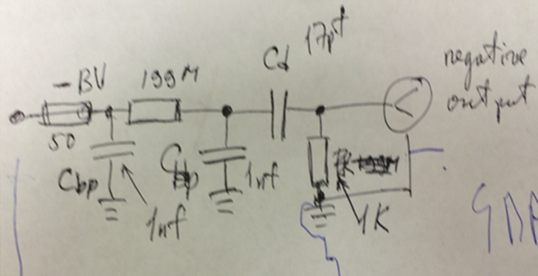
\includegraphics[width=0.45\textwidth]{plots/SiliconDiodeDiagram.png} 
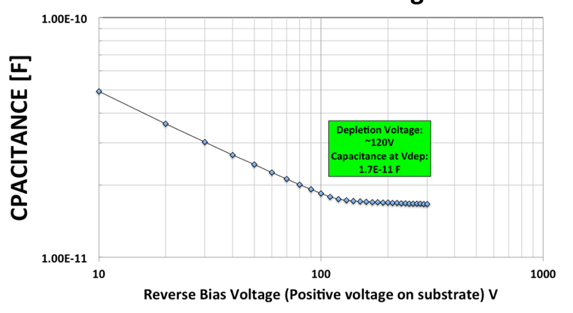
\includegraphics[width=0.45\textwidth]{plots/SiliconDiodeCV.png} 
\caption{The electrical schematics of the silicon diode is shown on the left. The measured
capacitance as a function of the applied bias voltage is shown on the right. } 
\label{fig:SiliconDiode} 
\end{figure} 


The silicon diode was placed inside a metal box of thickness $1.5$~cm. 
The HV was applied to the printed circuit board by a cable terminated by an SHV connector
at the other end. The silicon diode output signal is read out through an SMA connector attached 
to the box. The dark current was measured as a function of the bias voltage. The maximum value of the 
current at -500 V of the bias was less of $1$~nA. The silicon box and bench test setup are presented 
in Figure~\ref{fig:SiliconPad}. 

\begin{figure}[htbp] 
\centering
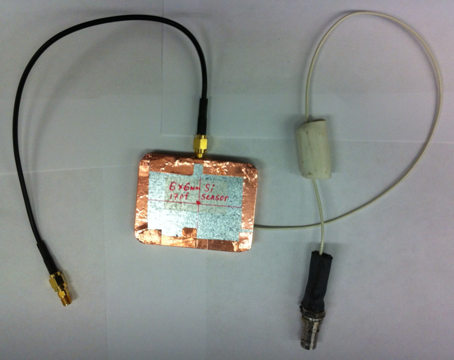
\includegraphics[width=0.45\textwidth]{plots/SiliconPadExternalView.png} 
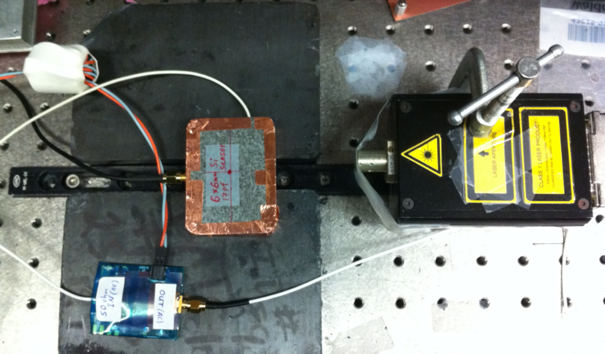
\includegraphics[width=0.45\textwidth]{plots/SiliconPadBench.png} 
\caption{External view of the box with silicon diode and PC board inside (left) and bench test setup (right).} 
\label{fig:SiliconPad} 
\end{figure} 


%TODO: this section is a bit weak...needs more details.
%TODO: We should put the photo of the circuit here


\section{Test-beam Setup and Experimental Apparatus }
\label{sec:tbeam}

% We need a better photograph of the testbeam setup. try to find it from phones.

We performed the test-beam measurements at the Fermilab Test-beam Facility (FTBF) which provided
proton beams from the Fermilab Main Injector accelerator at $120$~GeV, and secondary beams composed
of electrons, pions, and muons of energies ranging from $4$~GeV to $32$~GeV. A simple schematic diagram
of the experimental setup is shown in Figure~\ref{fig:BeamSchematicDiagram}. A small plastic scintillator 
of transverse dimensions $1.8$~mm$\times 2$~mm is used as a trigger counter to initiate the read out of
the data acquisition (DAQ) system. It is also used to constrain the transverse beam-spot to a small geometric area. 
Next, we place a stack of tungsten absorbers of various thicknesses for measurements at various
longitudinal locations within the electromagnetic shower. The silicon pad sensor is located within a metal
box covered by copper foil, and is placed immediately downstream of the absorber plates. Finally, a 
Photek 240 micro-channel plate photomultiplier detector~\cite{Anderson:2015gha, MCPFastCaloNIMA, Ronzhin2015288,Ronzhin201552} is placed furthest downstream, and serves to provide
a very precise reference timestamp. A photograph showing the various detector components is presented
in Figure~\ref{fig:BeamPhotoDiagram}. A differential Cherenkov counter is located further upstream of our
experimental setup and can provide additional particle identification capability. More details of
the experimental setup are described in our previous studies using the same experimental facility in
references~\cite{Anderson:2015gha, MCPFastCaloNIMA, Ronzhin2015288,Ronzhin201552}.

\begin{figure}[htbp] 
\centering
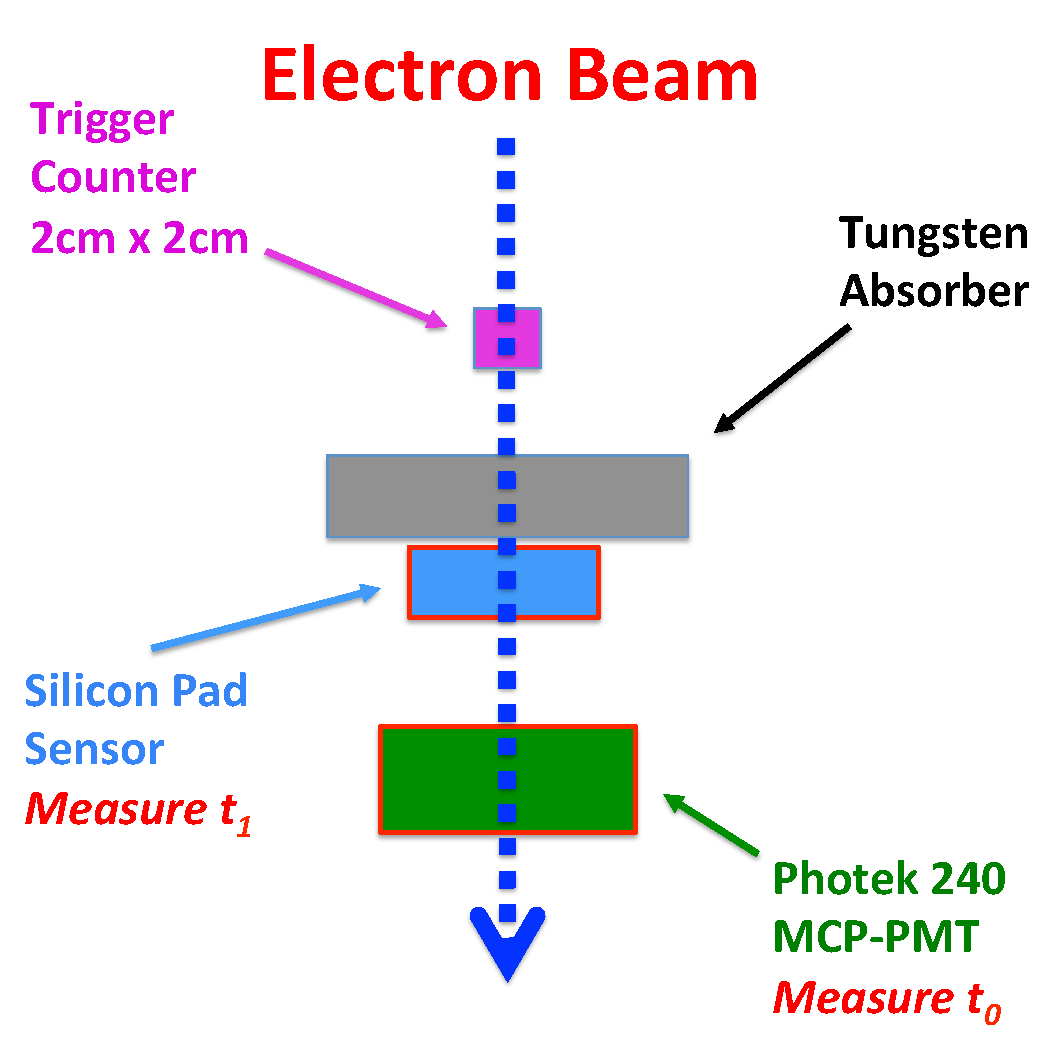
\includegraphics[width=0.65\textwidth]{plots/BeamSchematicDiagram.pdf} 
\caption{A schematic diagram of the test-beam setup is shown. } 
\label{fig:BeamSchematicDiagram} 
\end{figure} 

\begin{figure}[htbp] 
\centering
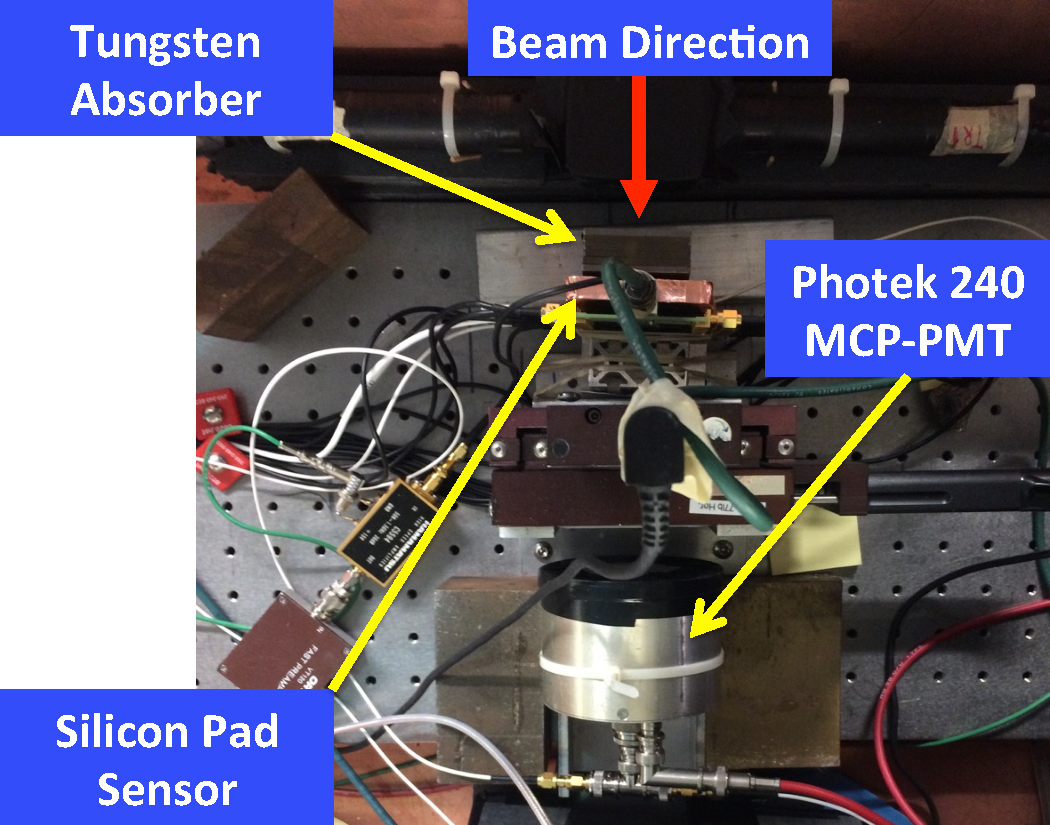
\includegraphics[width=0.65\textwidth]{plots/BeamPhotoDiagram.pdf} 
\caption{Test beam setup.} 
\label{fig:BeamPhotoDiagram} 
\end{figure} 

The DAQ system is based on the CAEN V1742 digitizer board~\cite{CAENDRS}, 
which provides digitized waveforms sampled at 5 GS/s. The metal box containing
the silicon sensor was located on a motorized X-Y moving stage allowing us to change the 
location of the sensor in the plane transverse to the beam at an accuracy better 
than $0.1$~mm. A nominal bias voltage of $500$~V was applied to deplete the silicon sensor.
The signals from the silicon sensor were amplified by two fast and high-bandwidth pre-amplifiers 
connected in series. The first amplifier is an ORTEC VT120C pre-amplifier, and the second
amplifier is a Hamamatsu C5595 amplifier. Using a pulse-generator, we measured the
combined amplification gain of the two amplifiers in series as a function of the input
signal amplitude and found some degree of non-linearity for typical signals
produced by the silicon sensor under study. The measured gain ranged from 
$200$ for signals with amplitude around $0.15$~mV to $650$ for signals with
amplitude around $10$~mV.

\section{Test Beam Measurements and Results} 
\label{sec:results} 

Measurements were performed using the secondary beam at the FTBF, which provides
a beam of electrons and pions. Beam energies ranging from 4 GeV/c$^2$ to 32 GeV/c$^2$
were used, for which the electron purity ranges between $70\%$ at the lowest
energy to about $10\%$ at the highest energy. Stacks of tungsten plates with
different thicknesses were placed immediately upstream of the silicon device in
order to measure the response along the longitudinal direction of the
electromagnetic shower. The transverse size of the tungsten plates allowed us to
fully cover the transverse size of the silicon device. The signals from the
silicon sensor and the Photek MCP-PMT are read out and digitized by the V1742
digitizer, and example signal waveforms are shown in Fig.~\ref{fig:pulses}.
The signal pulse in the silicon sensor has a rise time of about $1.5$~ns, and
a full pulse width of around $7$~ns. 

\begin{figure}[htbp] 
\centering
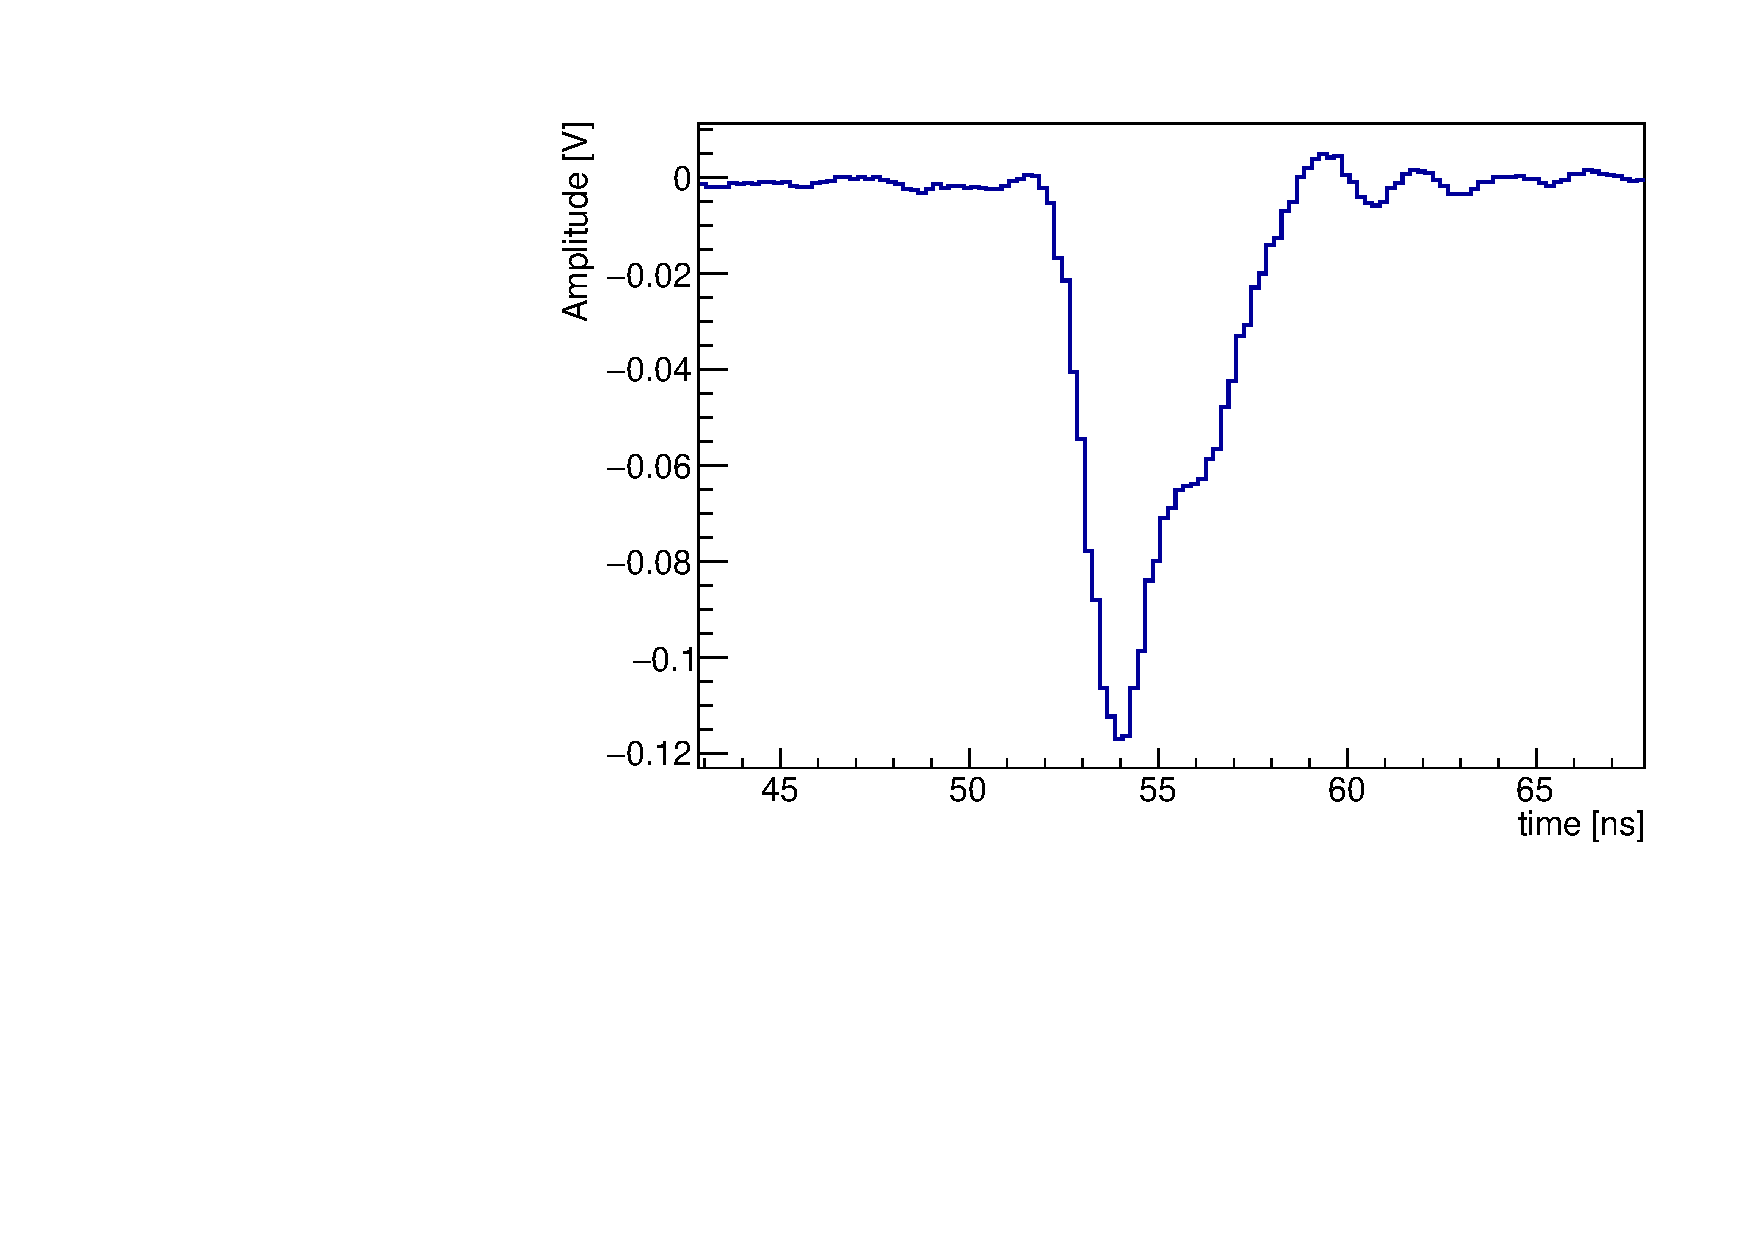
\includegraphics[width=0.45\textwidth]{plots/ExampleSiliconPadPulse_6X0_16GeV.pdf} 
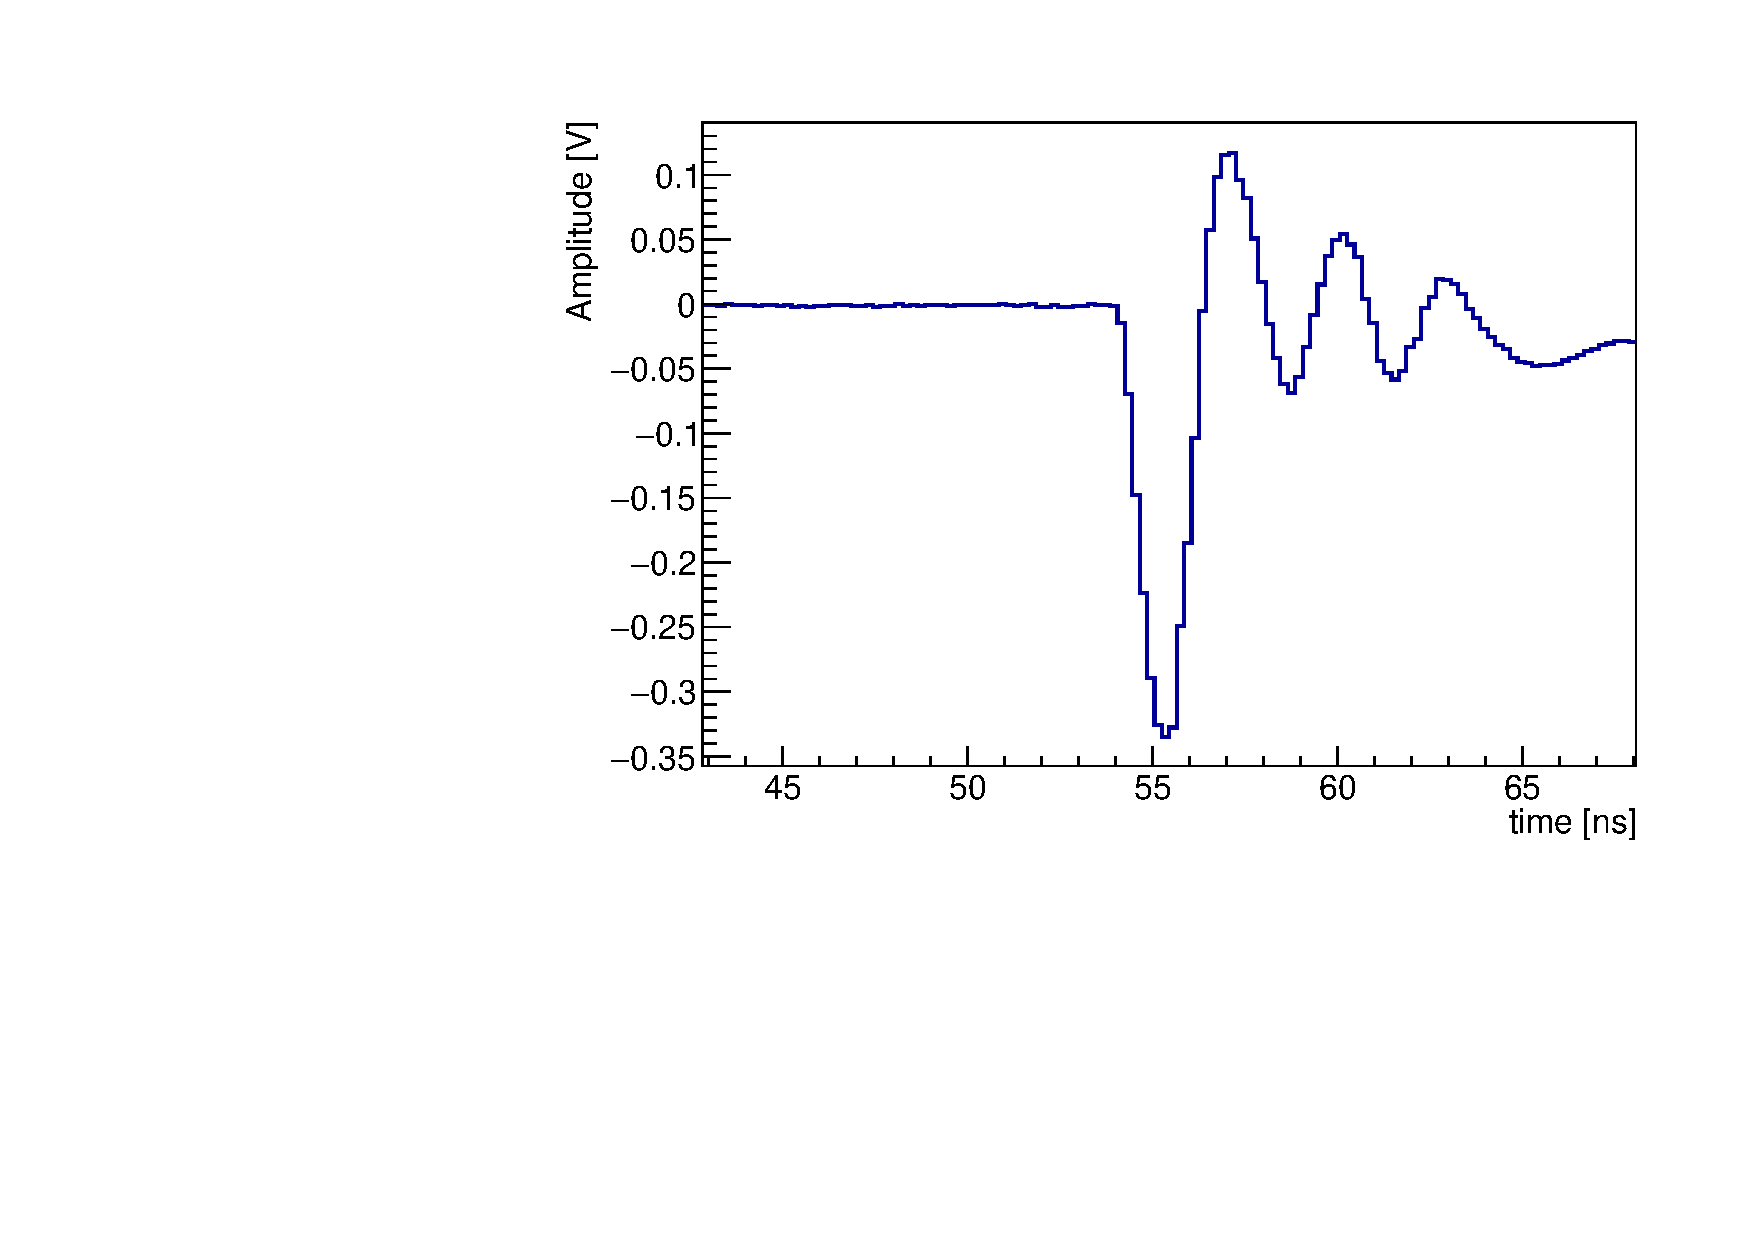
\includegraphics[width=0.45\textwidth]{plots/ExamplePhotekPulse.pdf} 
\caption{Examples of the signal pulse waveform for the silicon sensor (left) and the Photek MCP-PMT (right) digitized by CAEN V1742 digitizer board.} 
\label{fig:pulses} 
\end{figure} 

The raw waveforms are calibrated in both the voltage and time dimension using
known inputs from a pulse generator~\cite{Kim201467}. The total collected charge for each
signal pulse is computed by integrating a $10-$ns window around the peak of the
pulse. The time for the reference Photek MCP-PMT detector is obtained by fitting
the peak region of the pulse to a Gaussian function and the mean parameter of
the Gaussian is assigned as the timestamp. The time for signals from the silicon
sensor is obtained by performed a linear fit to the rising edge of the pulse and
the time at which the pulse reaches 30\% of the maximum amplitude is assigned as
its timestamp. We measured the ��electronic�� time resolution of the CAEN
V1742 digitizer as $\sim$4~ps and neglected this impact on the timing measurements
described below.

Electrons were identified using a combination of the gas Cherenkov counter
provided by the FTBF and the signal size in the Photek detector located further
downstream of the silicon sensor. Electromagnetic showers induced by electrons
produce significantly larger signals in the Photek MCP-PMT, while pions produce
a much smaller signal. After imposing the electron identification 
requirements the electron purity is between $80\%$ and $90\%$ for all beam
conditions. 

We begin by establishing the signal characteristics of a minimum-ionizing
particle (MIP) using beams of 120 GeV protons as well as 8 GeV electrons with no
absorbers upstream of the silicon pad sensor. To distinguish MIP signals from
noise, we collect data events of pure noise with no beam and random triggers.
The charge distribution for noise runs is presented in
Fig.~\ref{fig:noise}. As expected, the charge distribution for noise
runs is centered at 0, and the RMS is about $2$~fC. 

\begin{figure}[htbp] 
\centering
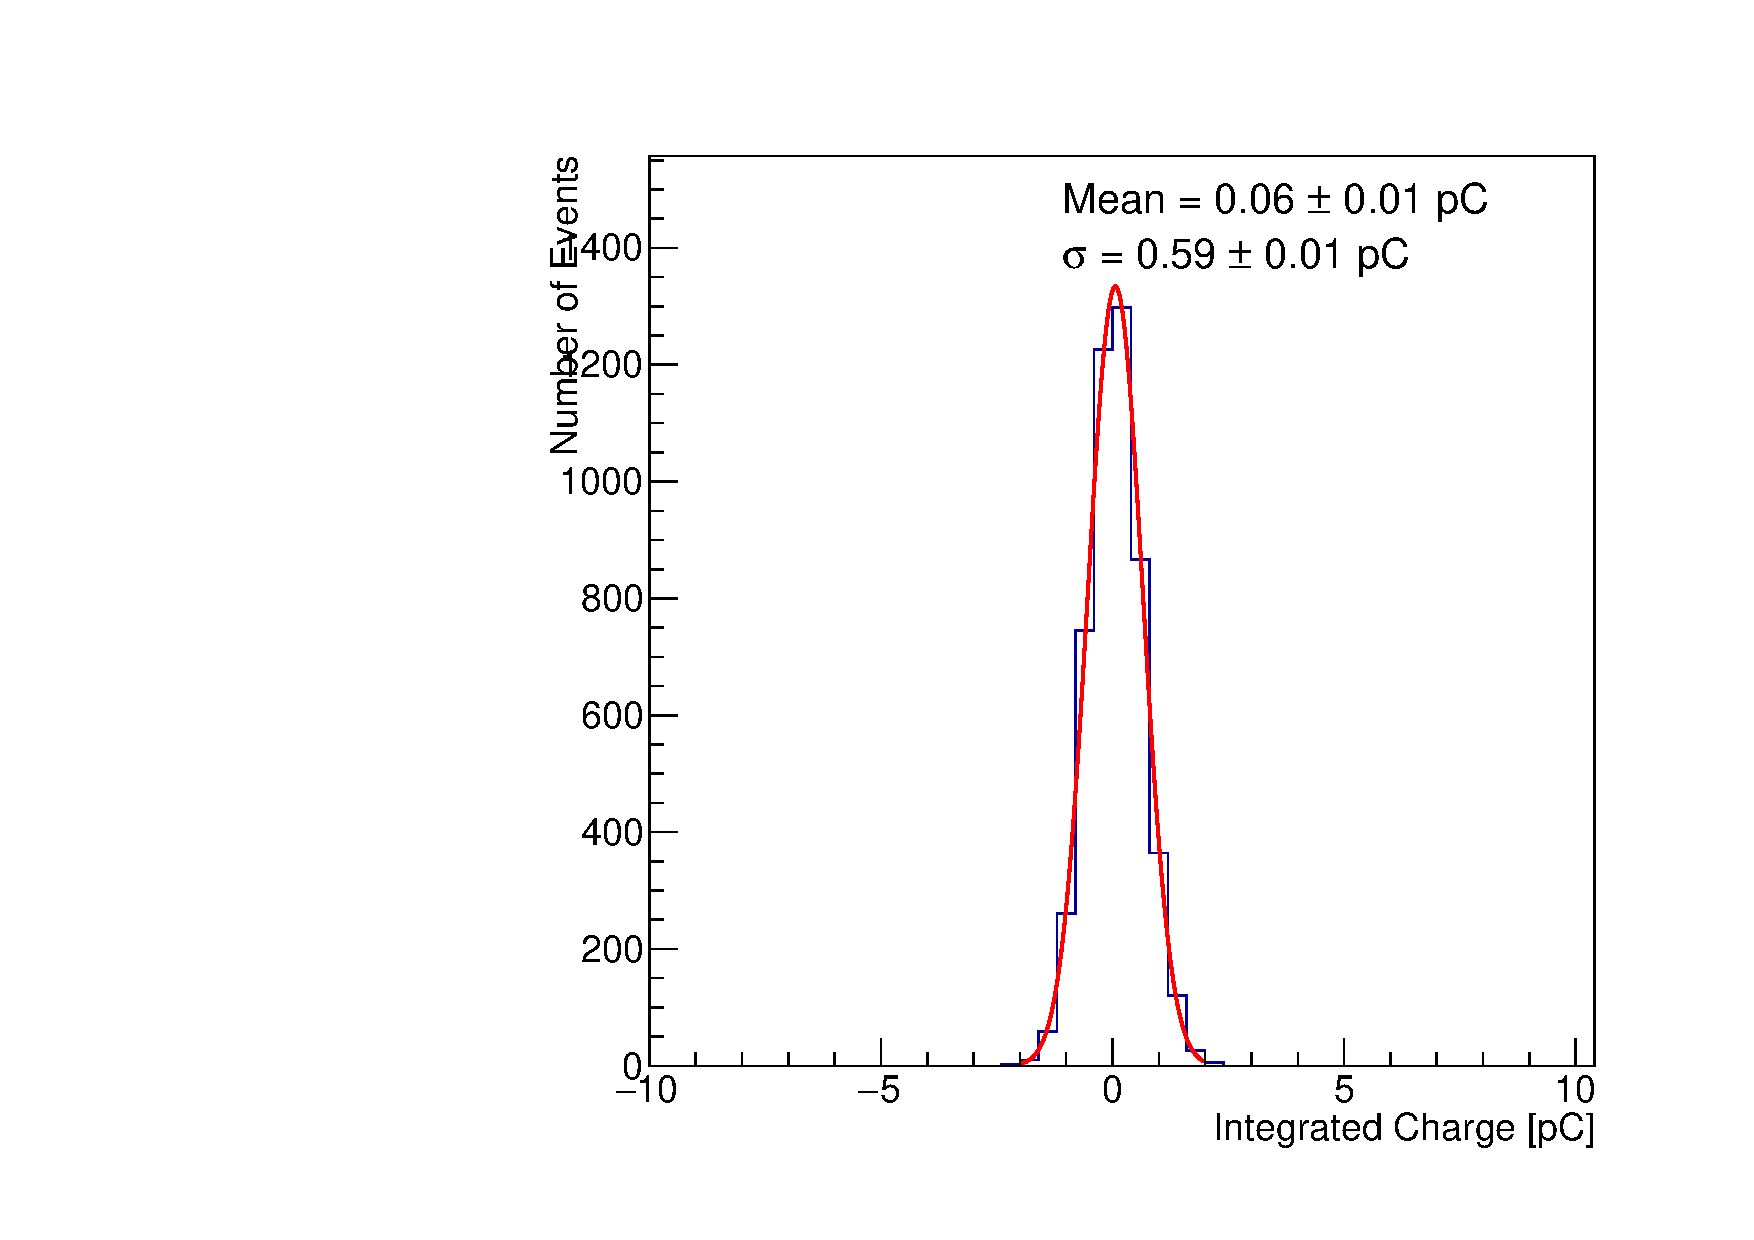
\includegraphics[width=0.45\textwidth]{plots/NoiseNoBeam_charge.pdf} 
\caption{The distribution of charge integrated in the silicon sensor is shown for randomly triggered 
data recorded with no beam. } 
\label{fig:noise} 
\end{figure} 

In Figure~\ref{fig:MIP}, we show the response of the silicon sensor to
the proton and electron beam without any absorbers upstream. We observe very similar
response for these two cases, and measure an integrated charge of $4.5$~fC and $5.0$~fC
for the proton and electron beams respectively. The measured charge takes into account
the response of the amplifiers and attenuators used, which were measured 
in the lab using a pulse generator in the full dynamic range relevant for the current study.
We expect that a MIP traversing a silicon sensor of thickness 300$\mu$m to produce roughly 32000 
electron-hole pairs, corresponding to a charge of about $5.1$~fC. Thus, our measured value
is in close agreement with expectations. Having established the absolute scale of the measured 
response using MIP's, in our remaining studies we normalize all charge measurements to the 
charge integrated in the silicon sensor for one MIP. 

\begin{figure}[htbp] 
\centering
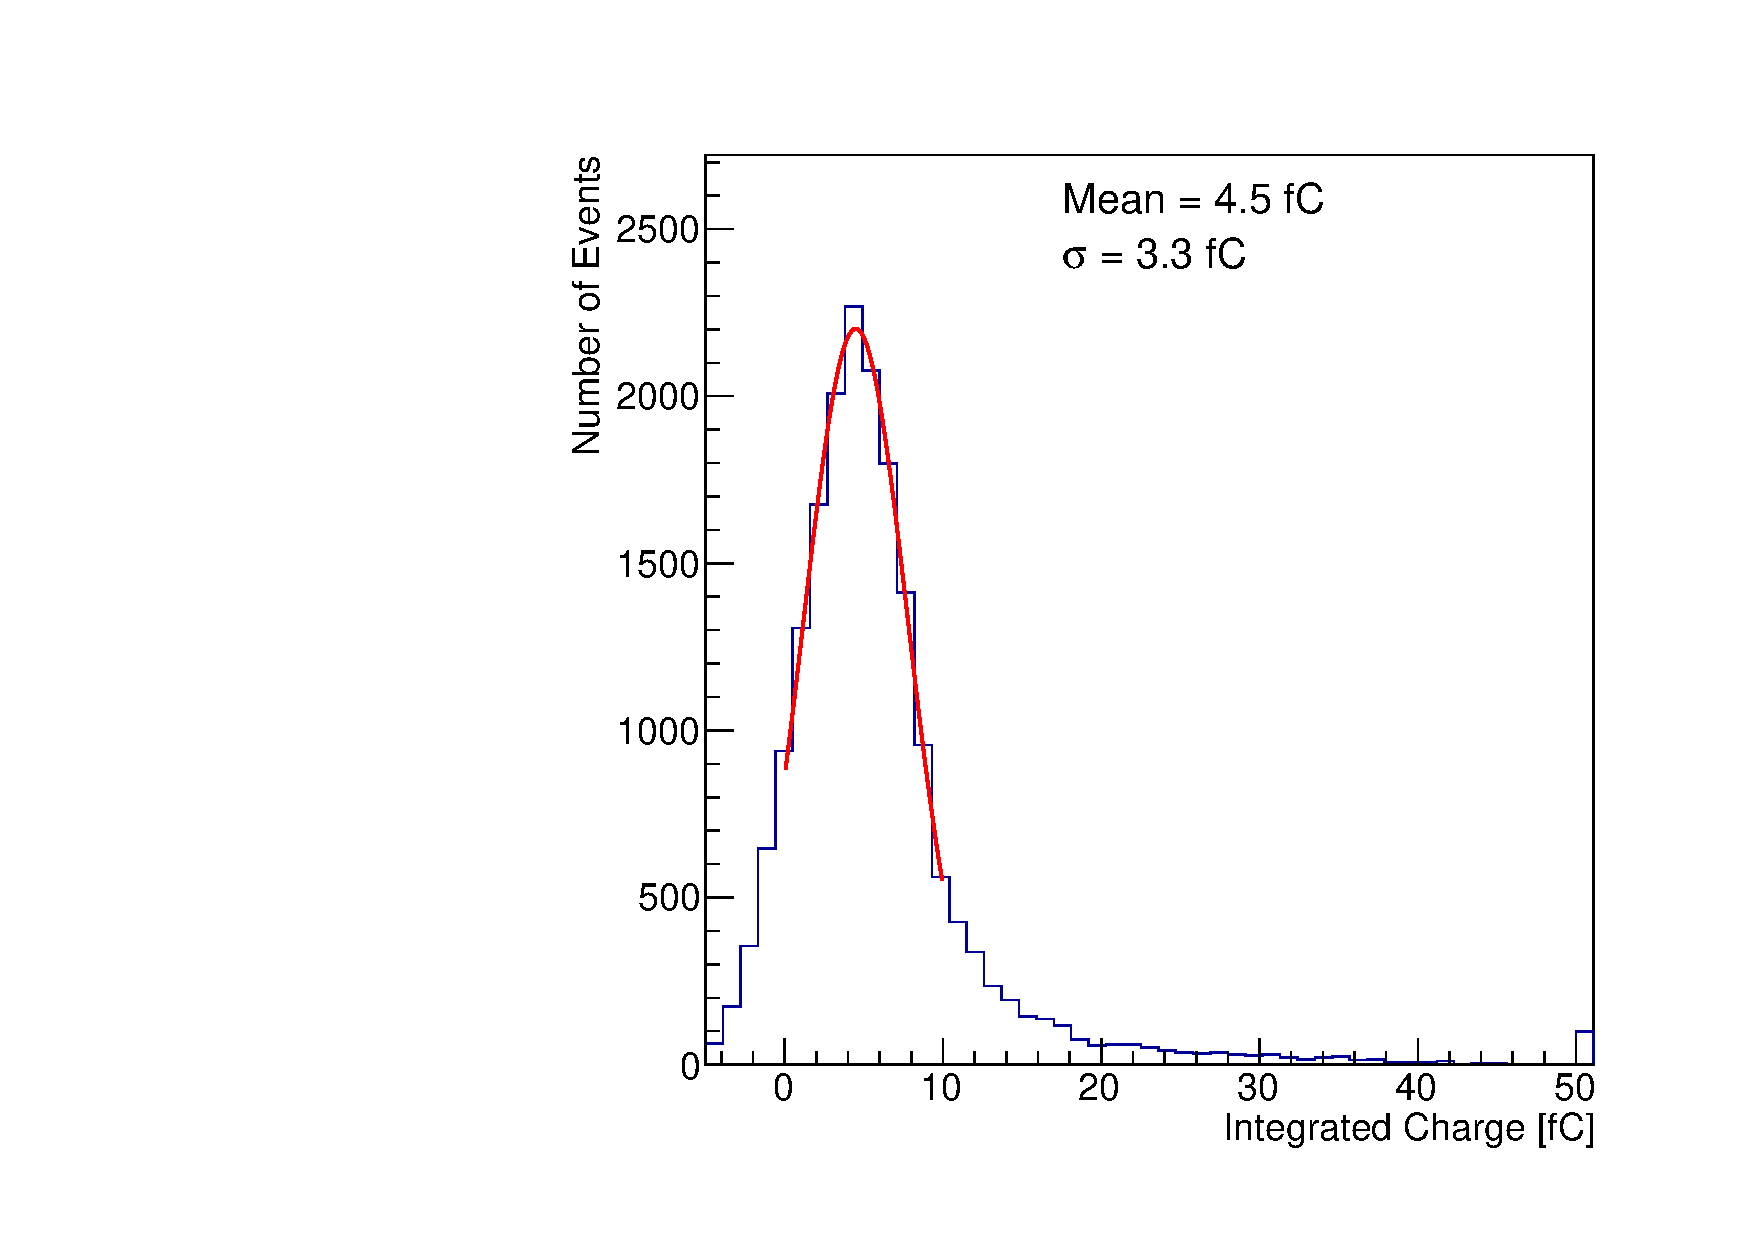
\includegraphics[width=0.45\textwidth]{plots/Proton_charge.pdf} 
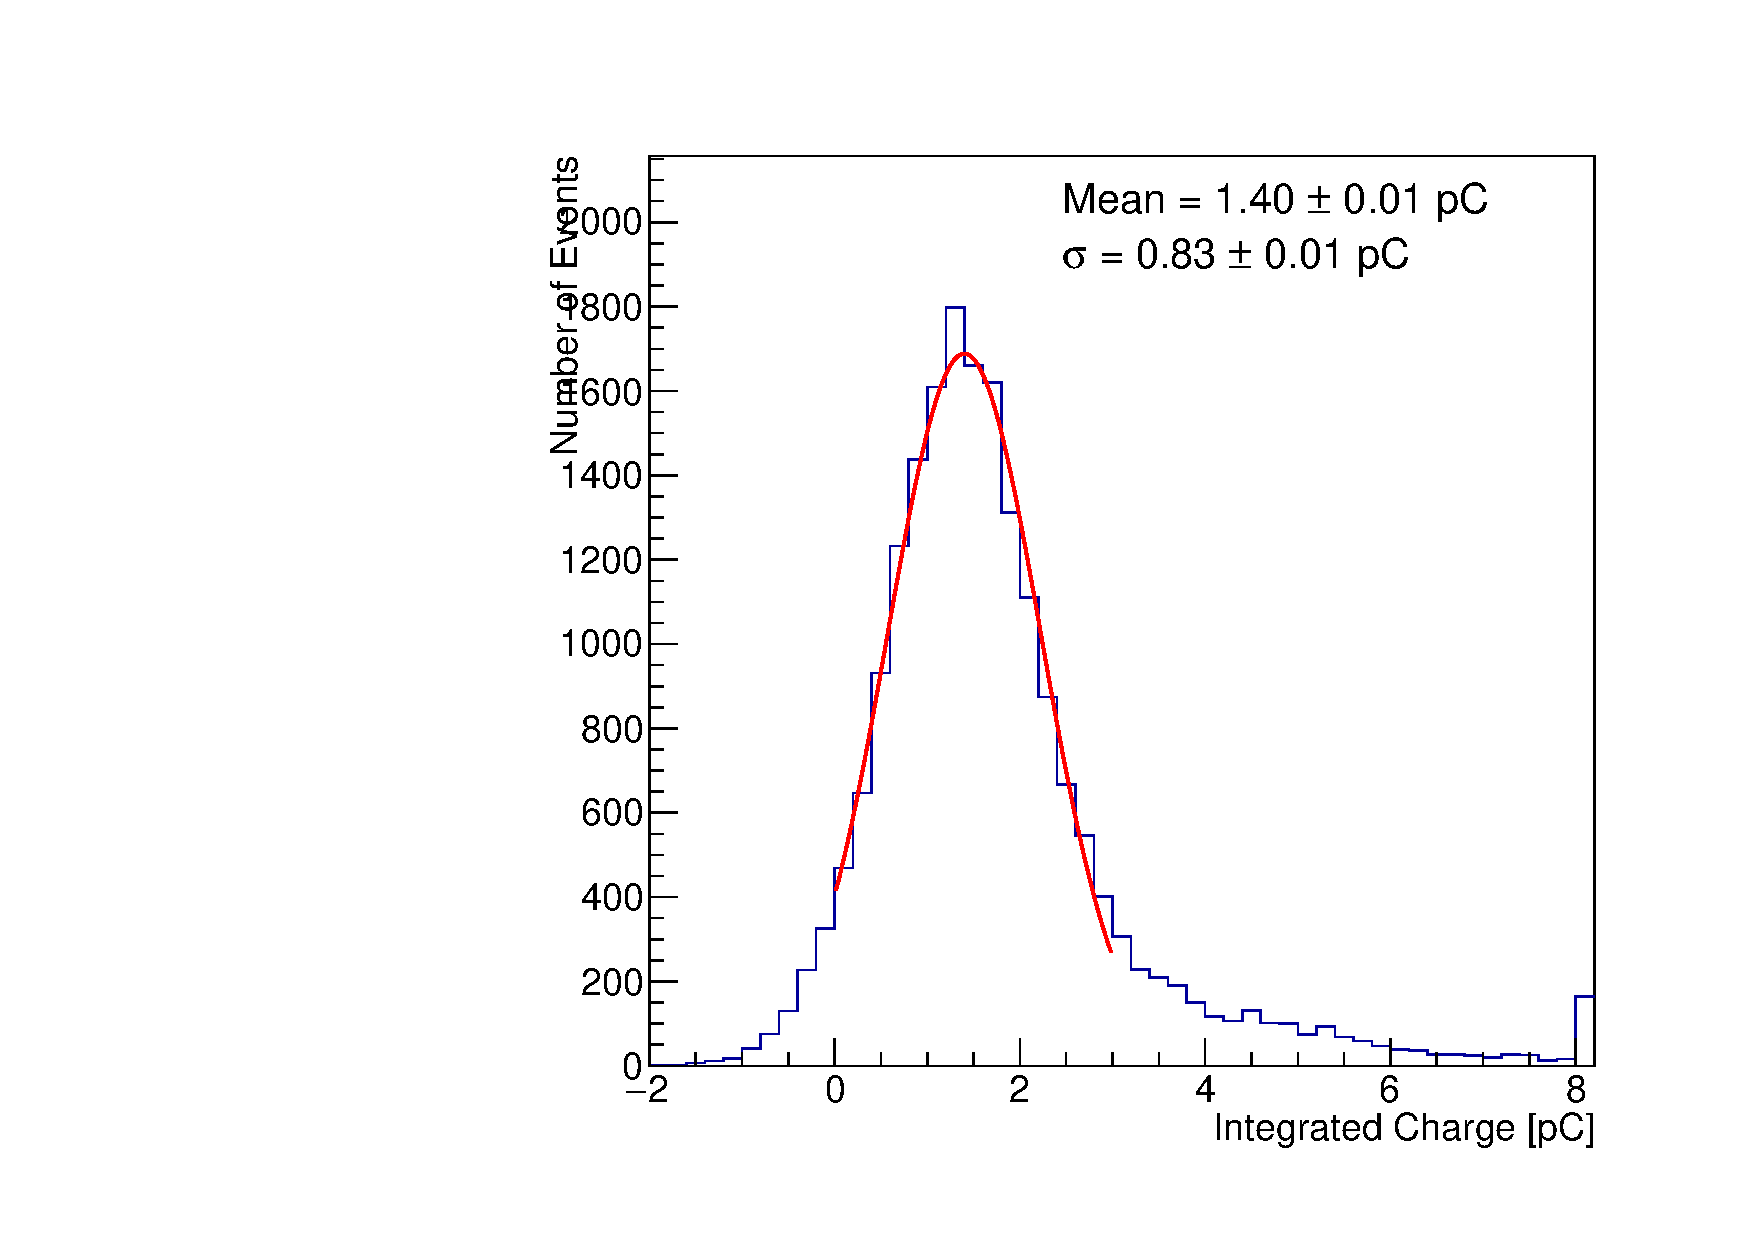
\includegraphics[width=0.45\textwidth]{plots/Electron_0X0_charge.pdf} 
\caption{The distribution of charge integrated in the silicon sensor is shown
for a beam of $120$~GeV protons (left) and $8$~GeV electrons (right) without
any absorber upstream of the silicon sensor. These conditions mimic the response
of the silicon sensor to a minimum-ionizing particle. 
} 
\label{fig:MIP} 
\end{figure} 

We study the response of the silicon sensor to electron beams of various energies after
6 radiation lengths of tungsten absorber. The silicon sensor is expected to be
sensitive to the number of secondary electrons produced within the electromagnetic
shower, and therefore its response is expected to scale up with higher incident
electron energy. In Figure~\ref{fig:ChargeDistributionExample}, we show
an example of the integrated charge distribution measured in the silicon sensor
after 6 radiation lengths of tungsten for $32$~GeV electrons. We plot the mean 
and RMS of these distributions as a function of incident electron beam energy
in Figure~\ref{fig:MIPVsEnergy}. The uncertainties plotted show the RMS
of the charge distribution. We observe a fairly linear depedence between
the measured charge and the incident beam energy, for beam energies
between $4$~GeV and $32$~GeV. 

\begin{figure}[htbp] 
\centering
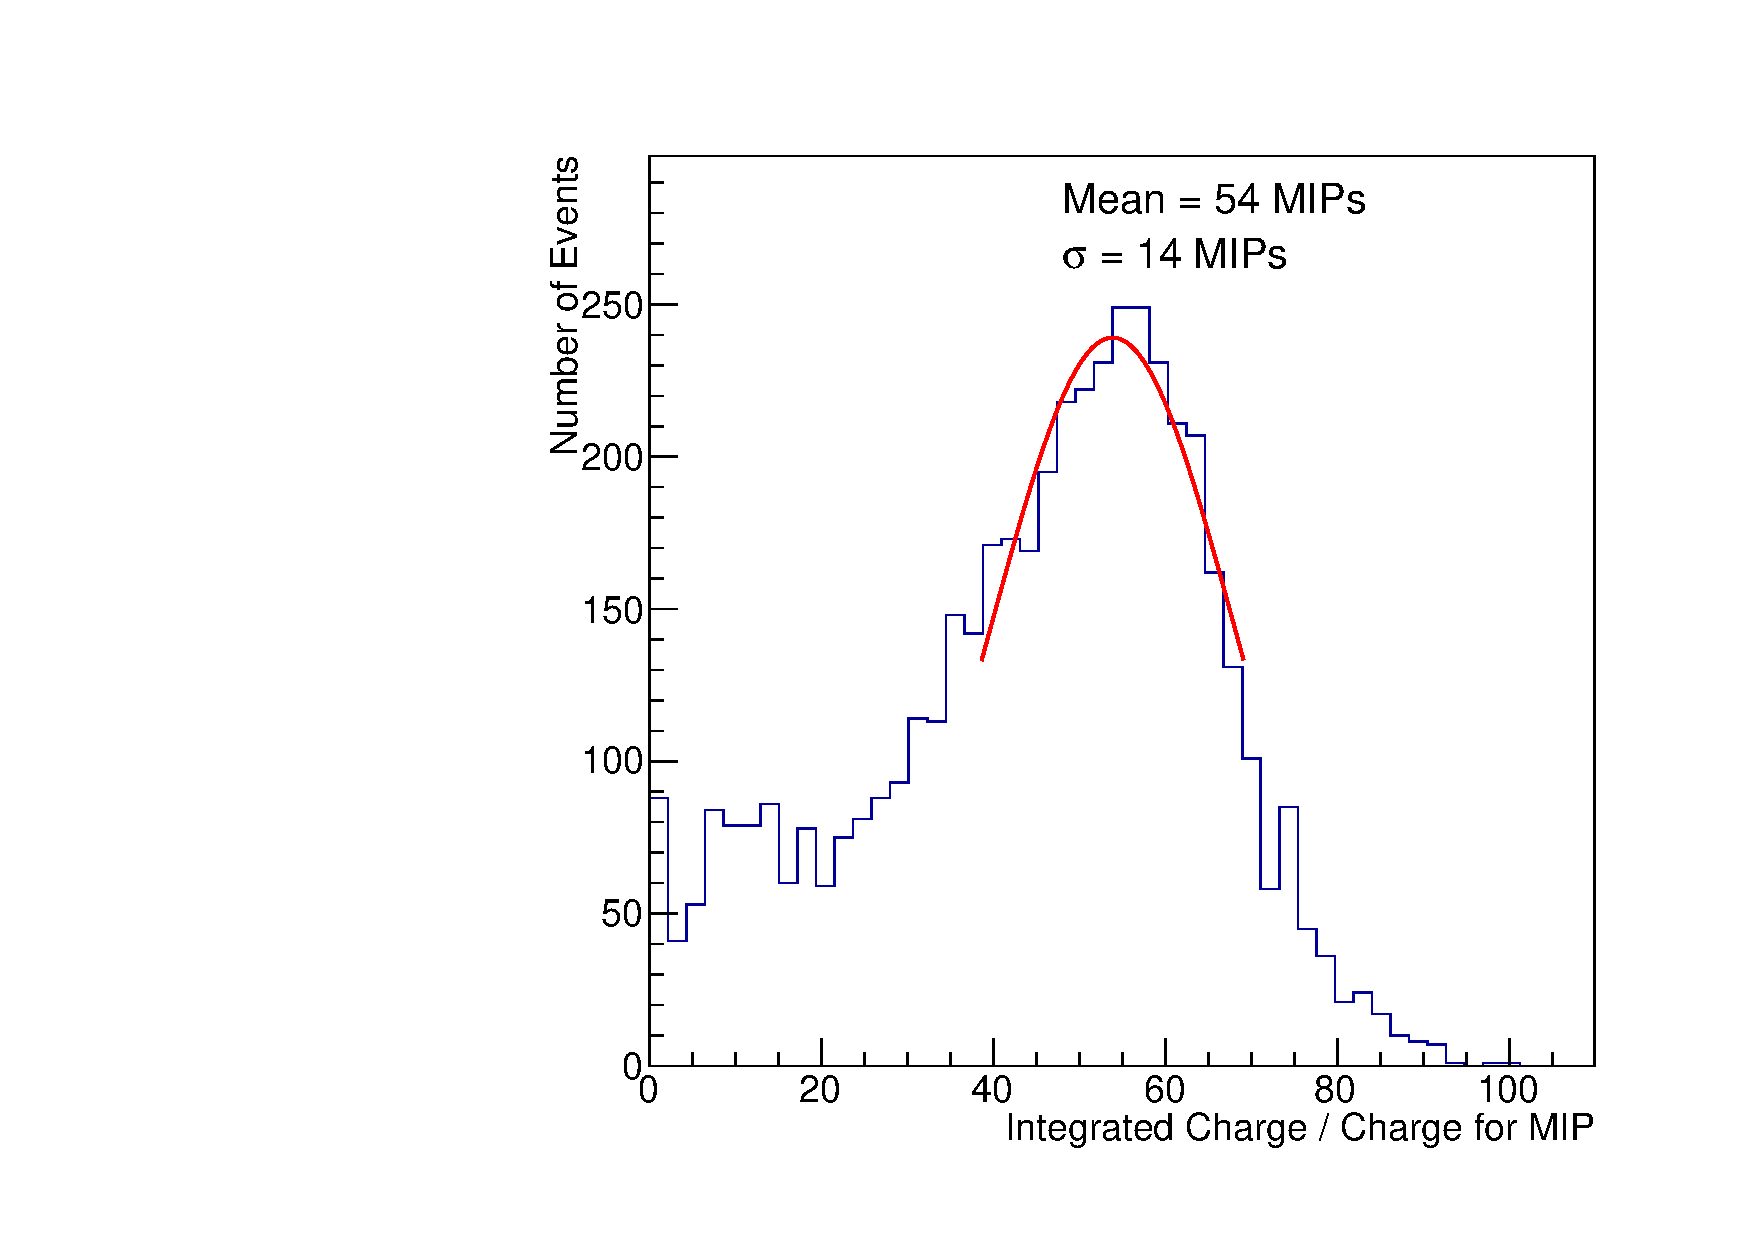
\includegraphics[width=0.49\textwidth]{plots/Electron_6X0_32GeV_chargeMIP.pdf} 
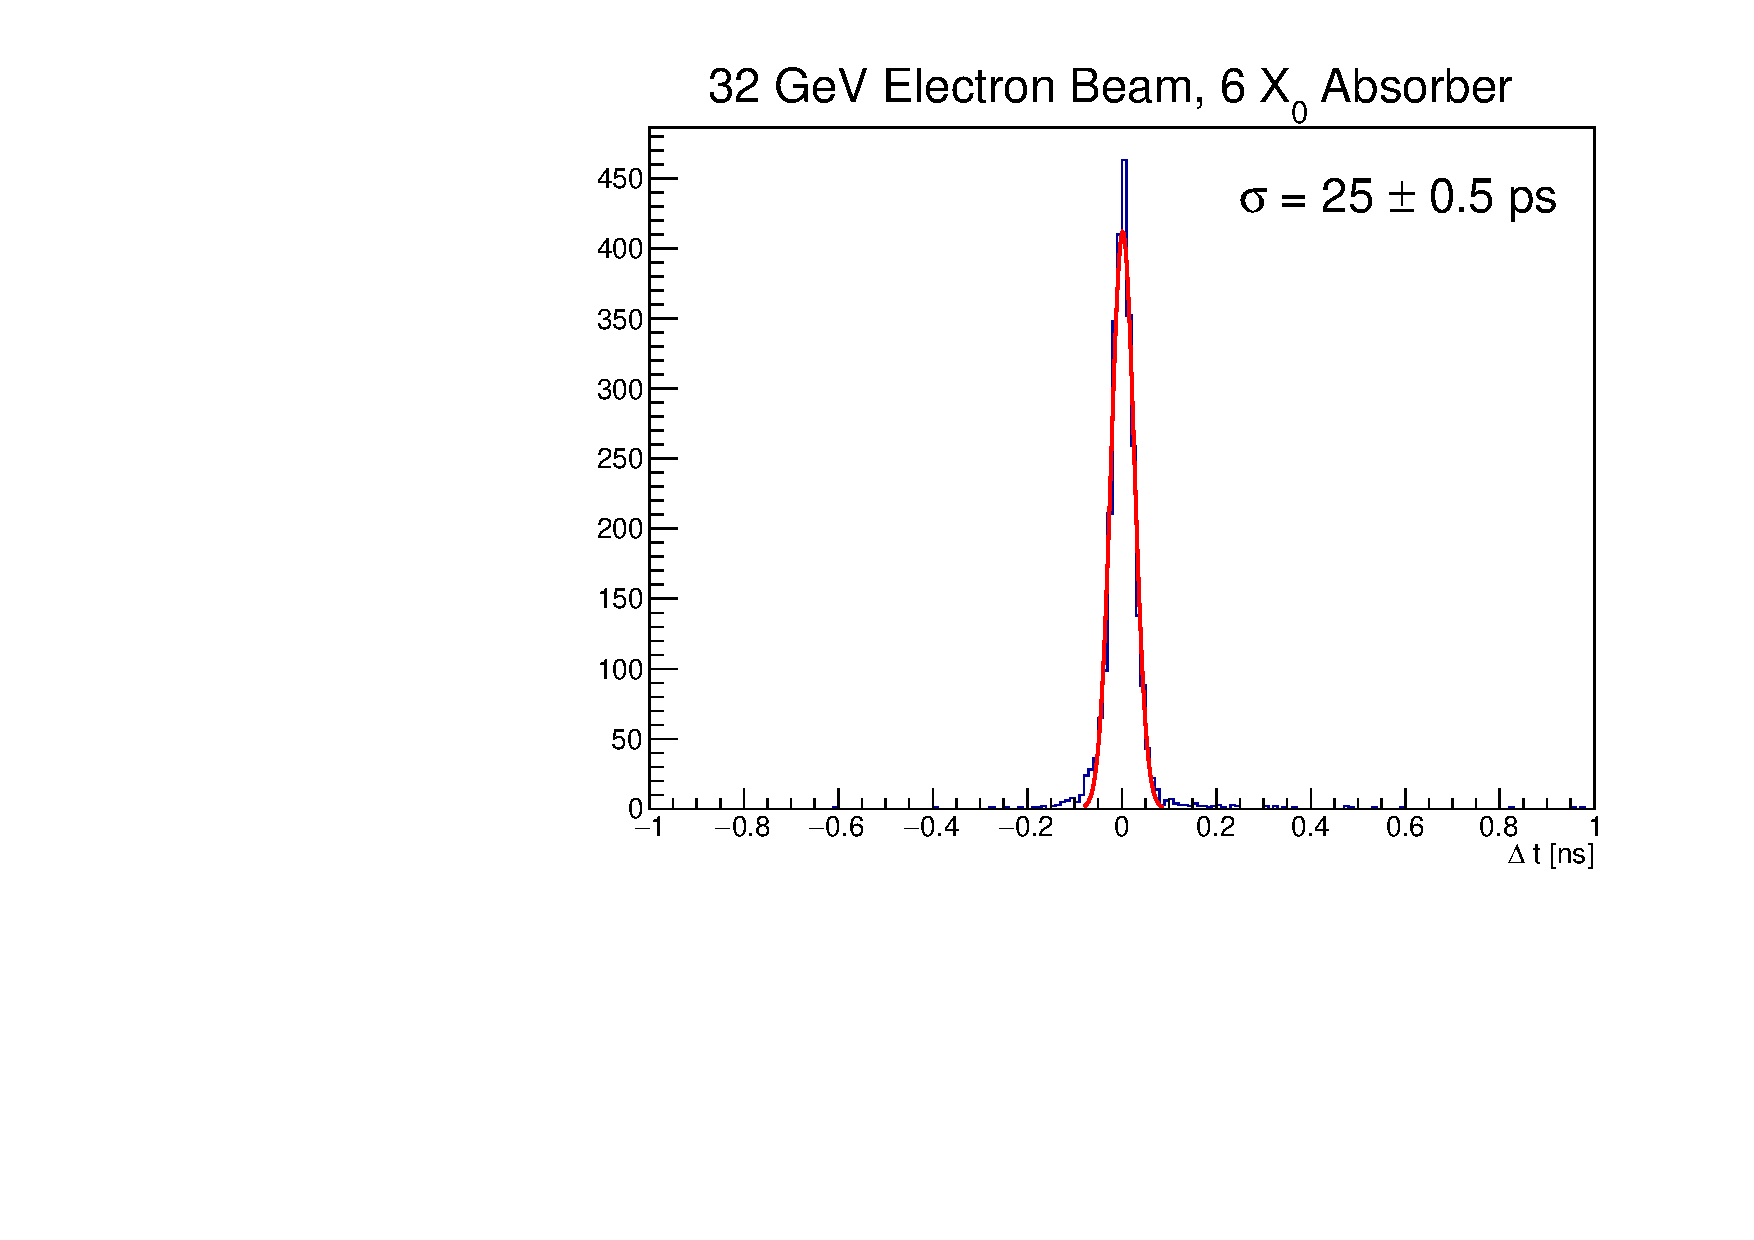
\includegraphics[width=0.50\textwidth]{plots/deltaT_32GeV_6X0.pdf} 
\caption{ An example of the distribution of integrated charge in the silicon sensor is 
shown in units of the charge measured for MIP's. A 32 GeV electron beam is used, and the
silicon sensor is placed after 6 radiation lengths of tungsten absorber.} 
\label{fig:ChargeDistributionExample}
\end{figure}

\begin{figure}[htbp] 
\centering
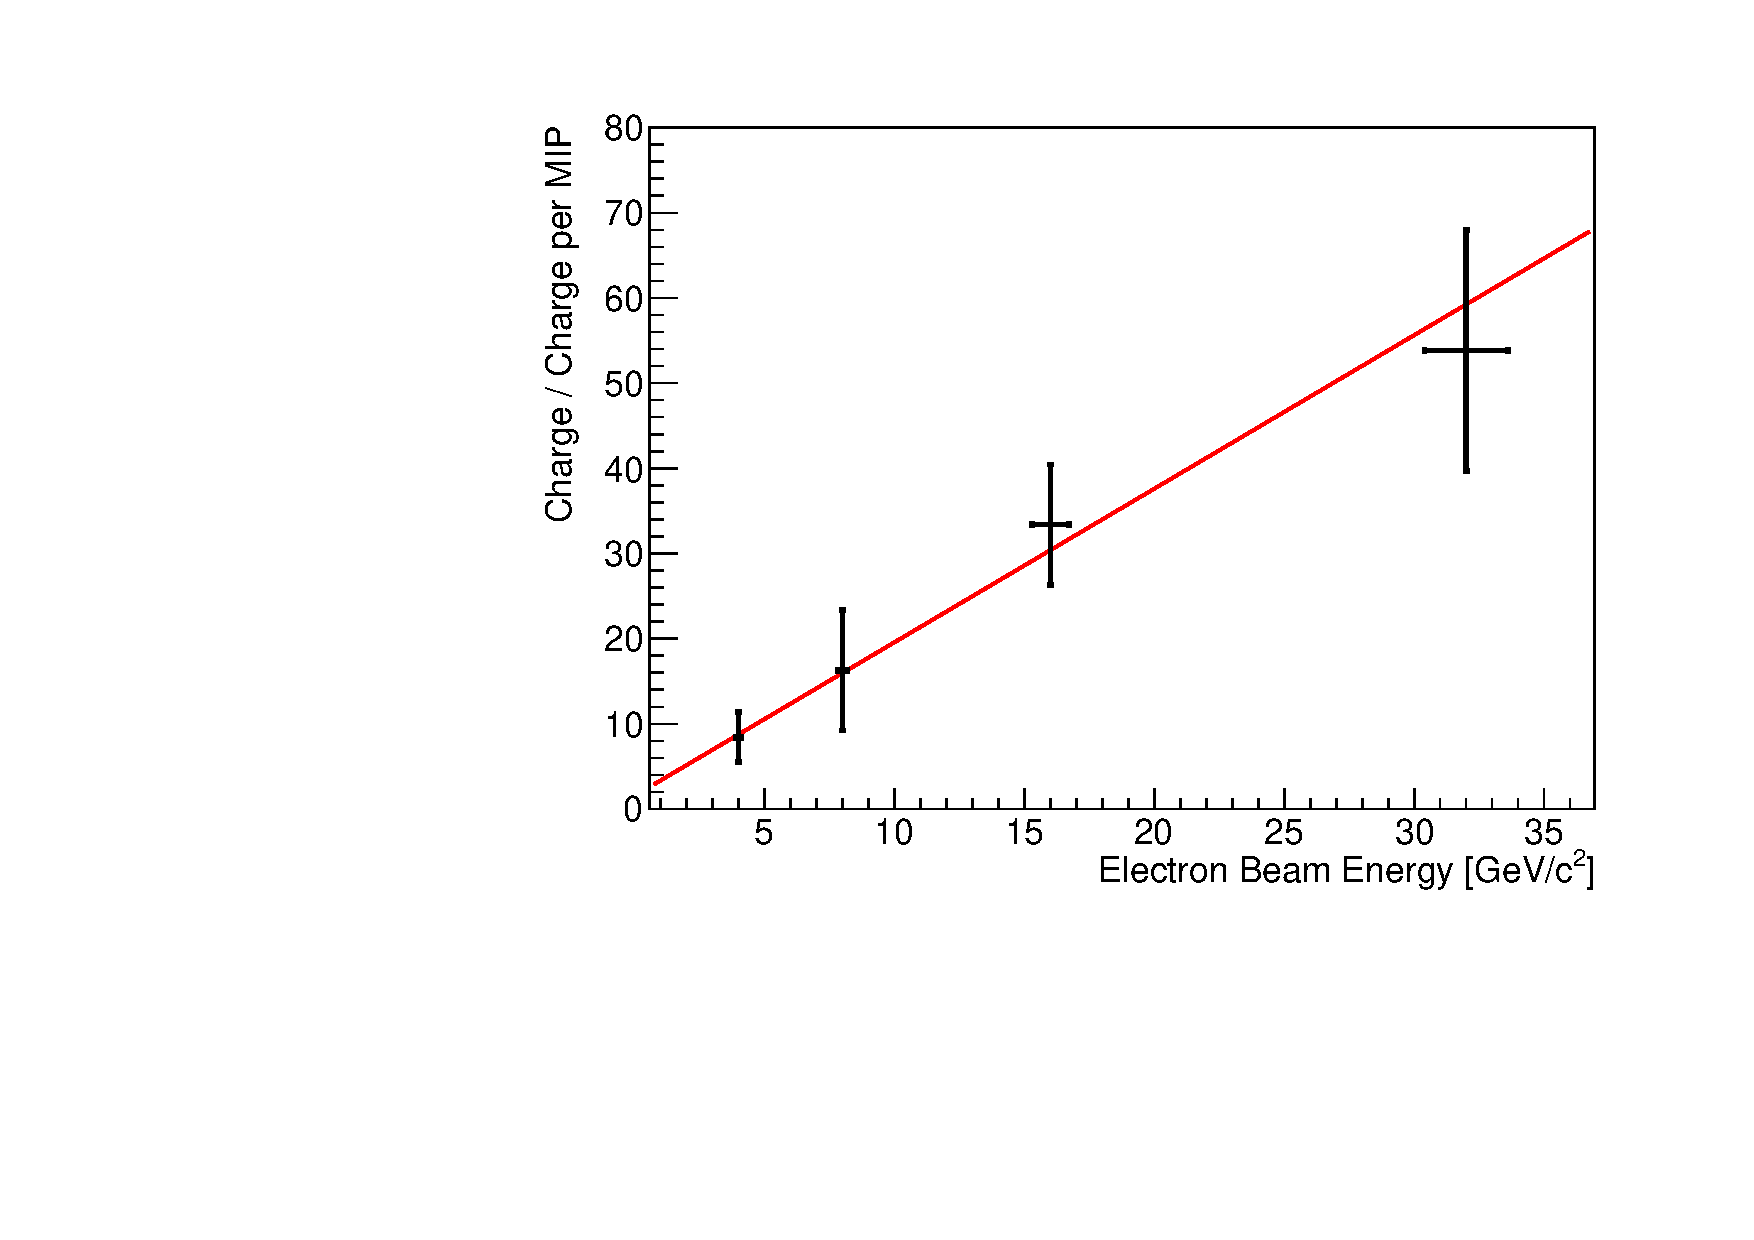
\includegraphics[width=0.49\textwidth]{plots/MIPVsEnergyAt6X0.pdf} 
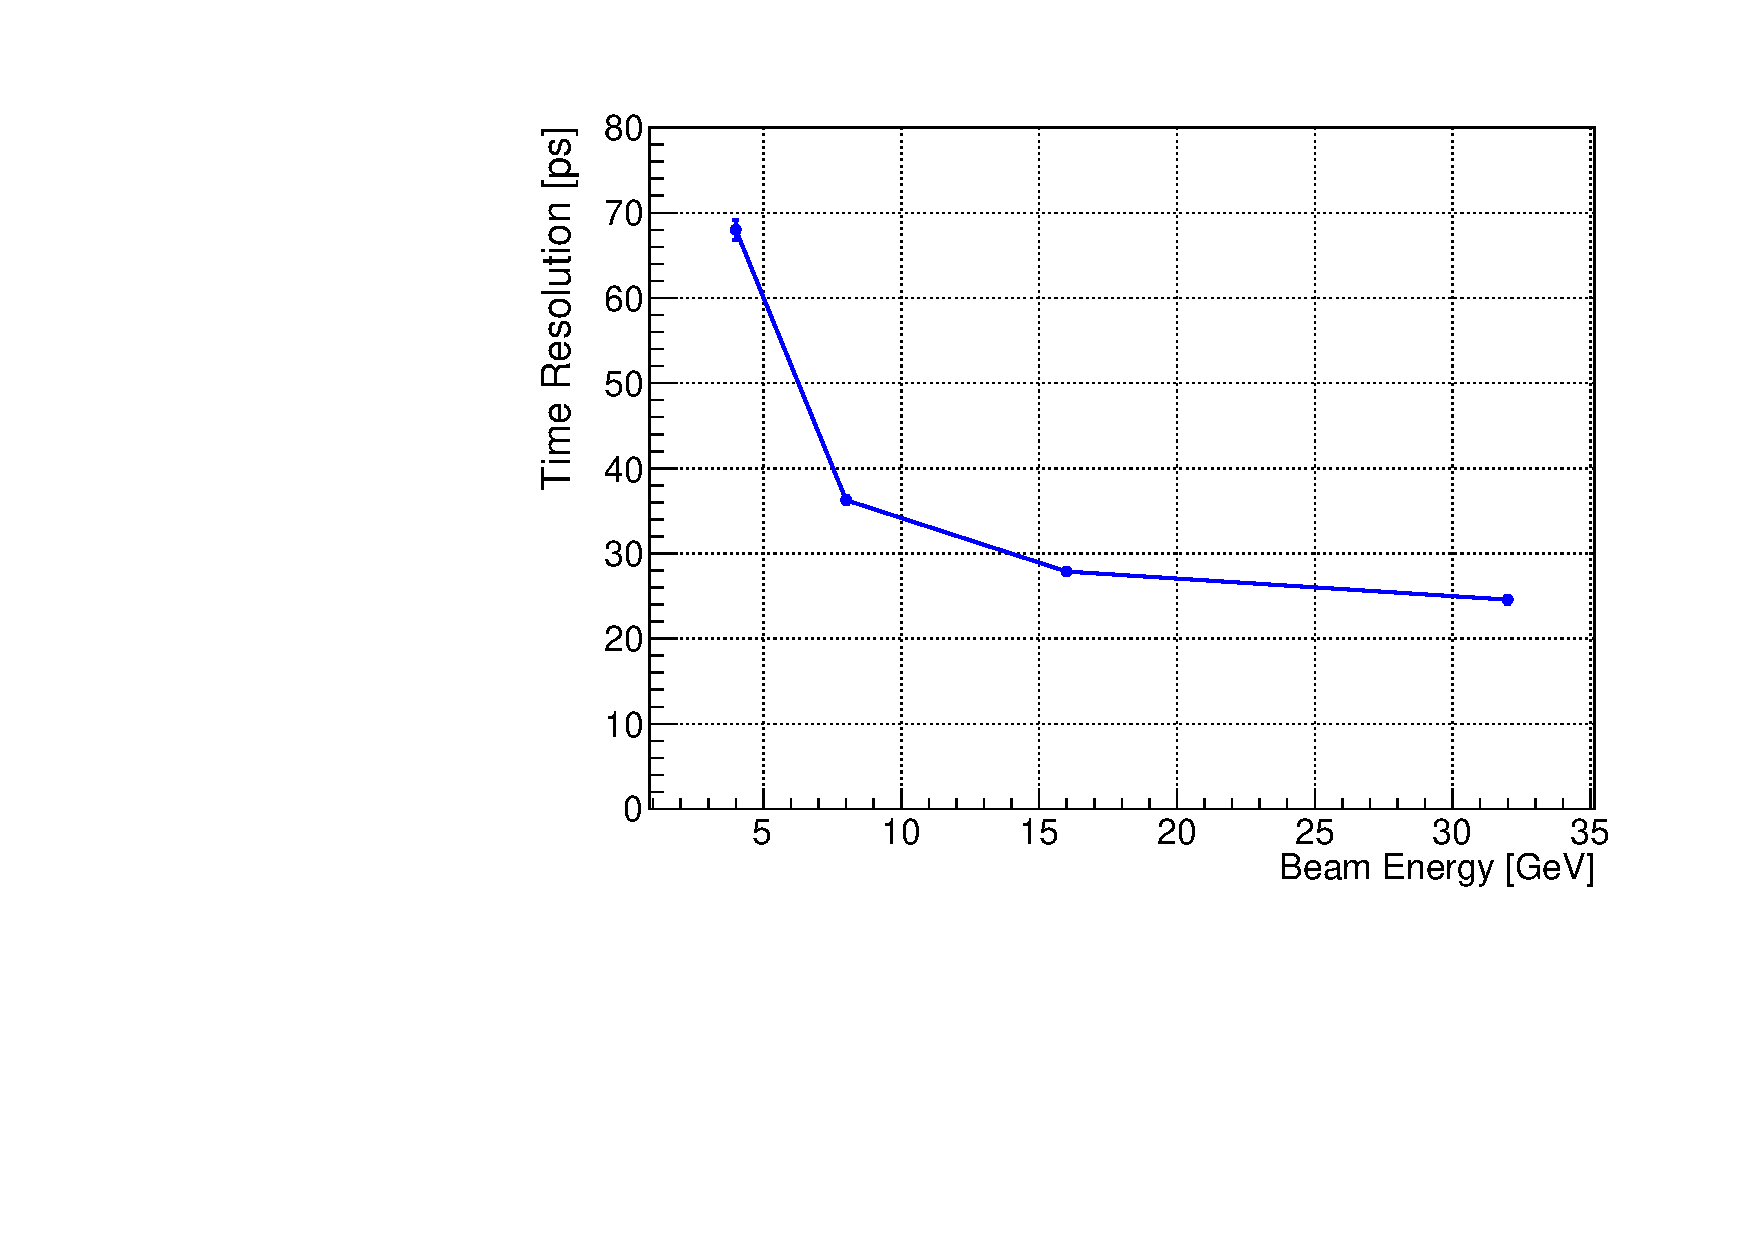
\includegraphics[width=0.50\textwidth]{plots/SigmaT_vs_BeamEnergy_lin30Stamp.pdf} 
\caption{On the left, the integrated charge in the silicon sensor expressed in units of the 
charge measured for MIP's is shown as a function of the electron beam energy. The uncertainty
bands show the RMS of the measured charge distribution. The red line is the best fit to a 
linear function. On the right, the measured time resolution between the silicon sensor and the 
Photek MCP-PMT reference is shown as a function of the electron beam energy.
} 
\label{fig:MIPVsEnergy} 
\end{figure} 

We also measure the time resolution between the silicon sensor and the Photek MCP-PMT.
An example of the time of flight distribution is shown on the right of 
Figure~\ref{fig:ChargeDistributionExample} for $32$~GeV electrons after 6 radiation
lengths of tungsten. The dependence of the measured time resolution on the beam
energy is shown on the right of Figure~\ref{fig:MIPVsEnergy}. We observe an improvement
in the time resolution as beam energy increases, and achieve a time resolution of $23$~ps
for the $32$~GeV electron beam. 

Furthermore, we study the response and time resolution of the silicon sensor
along the longitudinal direction of the shower development. We measure the
integrated charge and the time resolution as a function of the absorber thickness
and present the results in Figure~\ref{fig:MIPVsAbsorberAt8GeV}. A typical 
longitudinal shower profile is observed, consistent with previous studies performed
using a secondary emission calorimter prototype based on MCP's~\cite{MCPShowerMaxPaper},
as well as independent studies of silicon-based calorimeter prototypes~\cite{Muhuri201424}.
We also observe that the time resolution improves as the shower develops towards its 
maximum in the longitudinal direction.

\begin{figure}[htbp] 
\centering
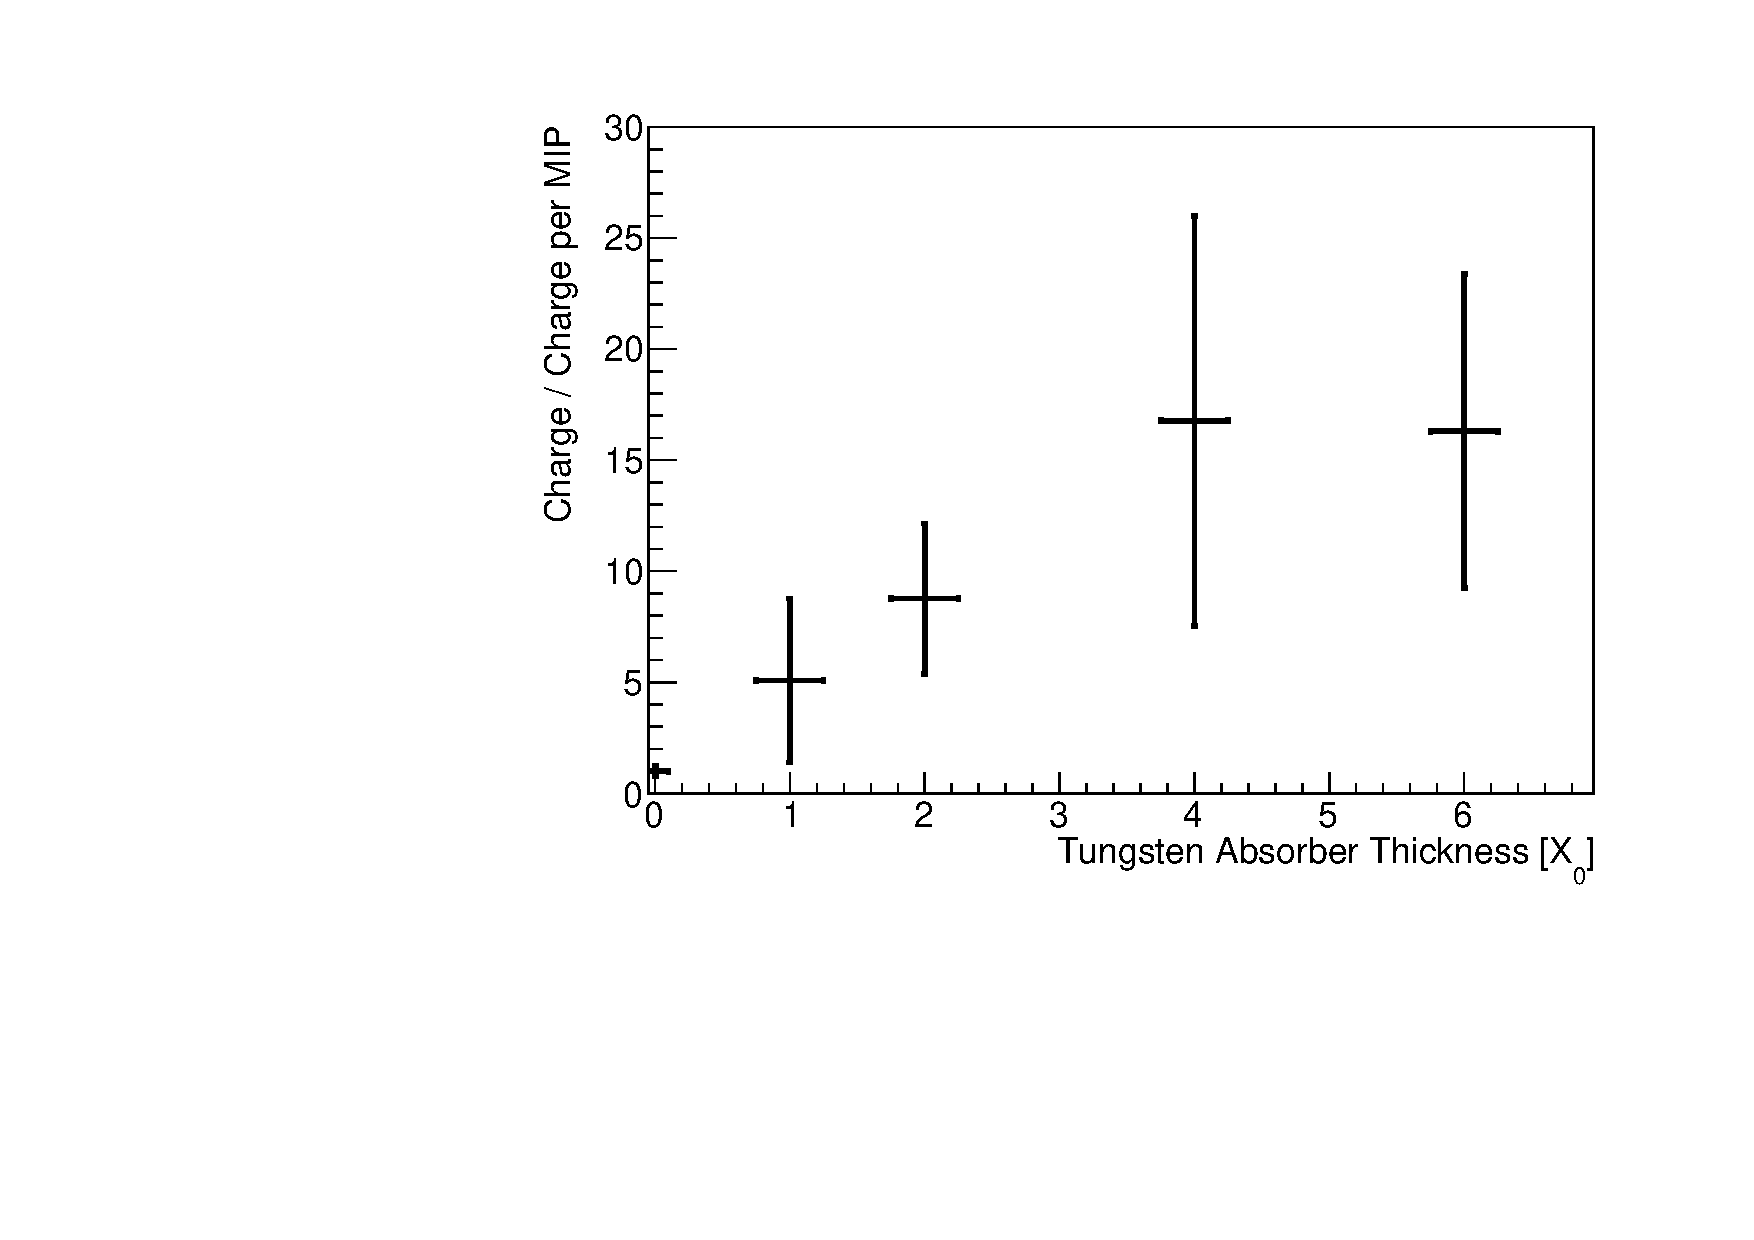
\includegraphics[width=0.49\textwidth]{plots/MIPVsAbsorberAt8GeV.pdf} 
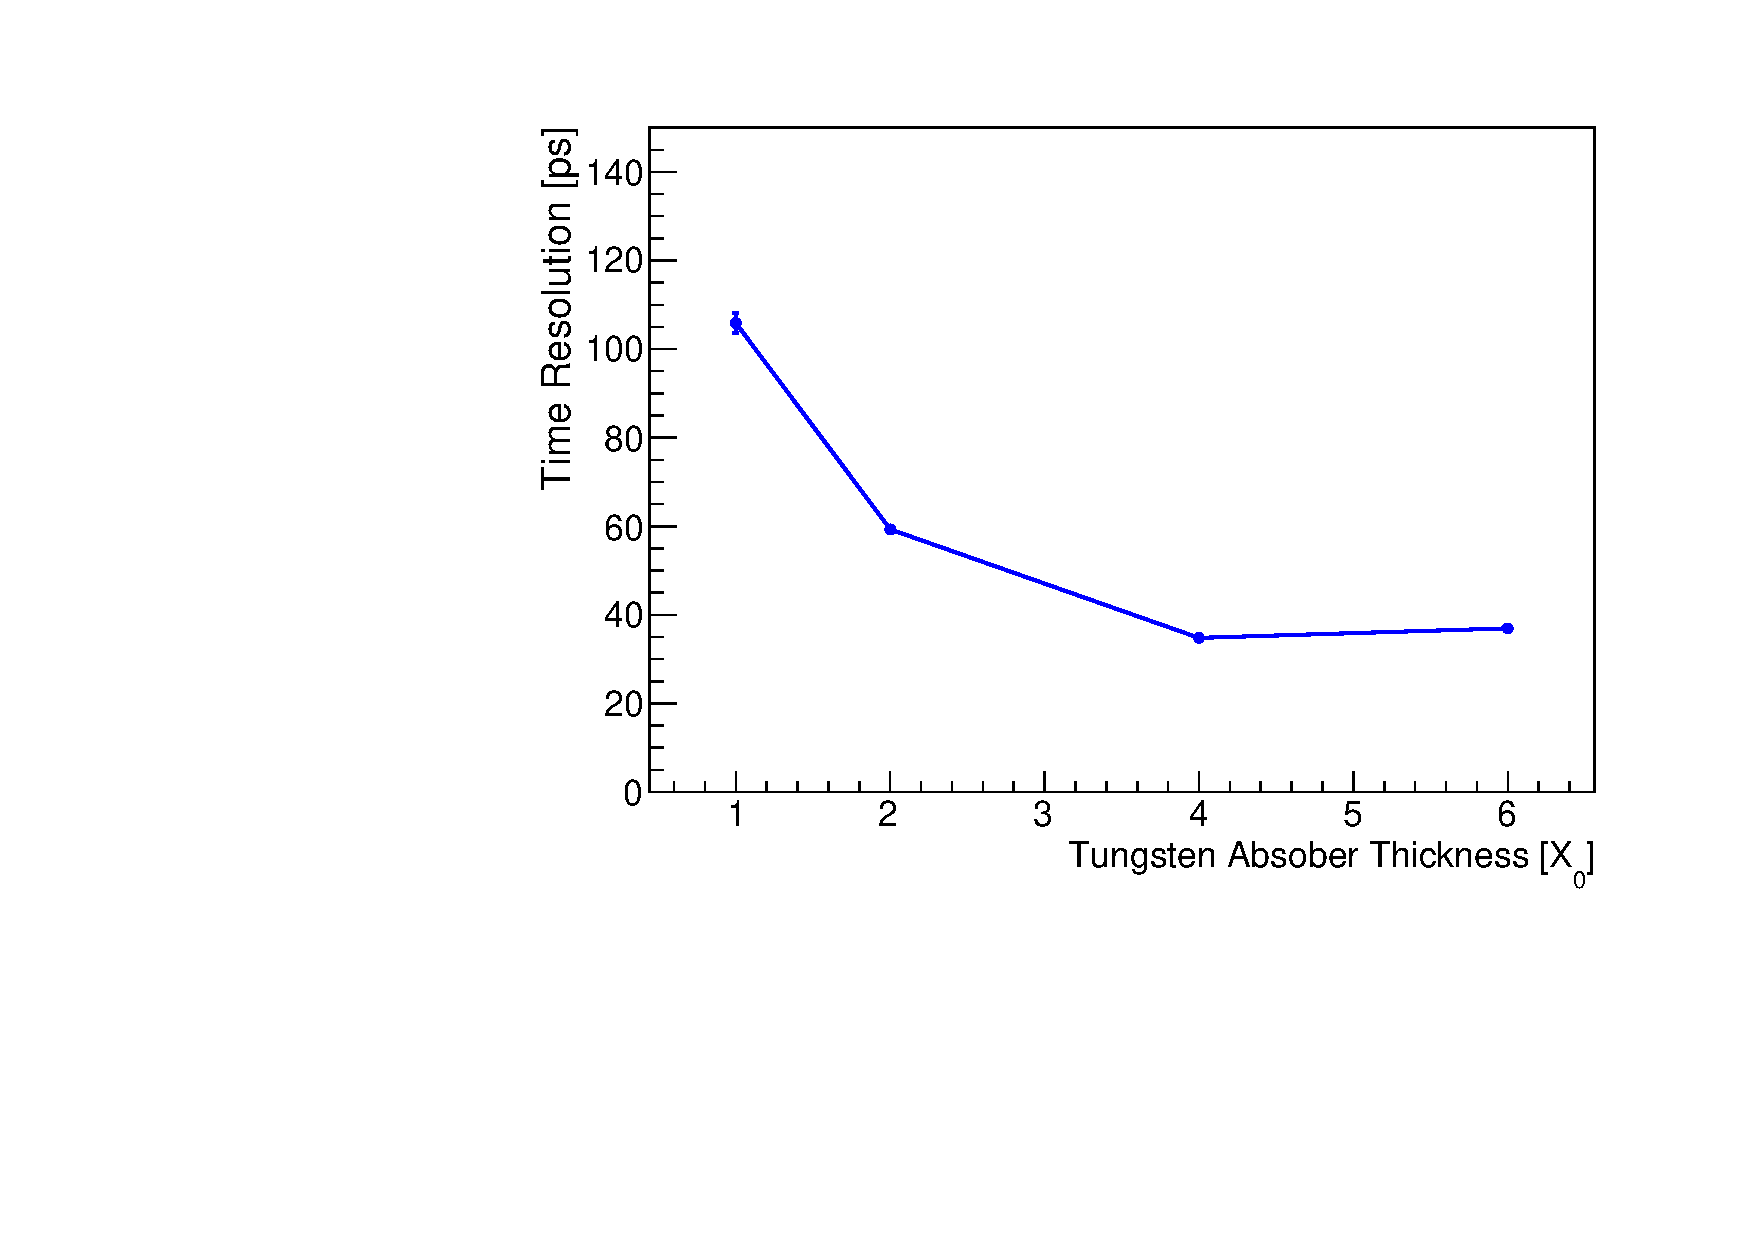
\includegraphics[width=0.5\textwidth]{plots/SigmaT_vs_X0_lin30Stamp.pdf} 
\caption{On the left, the integrated charge in the silicon sensor expressed in units of the 
charge measured for MIP's is shown as a function of the absorber (W) thickness measured in
units of radiation lengths ($X_{0}$). The uncertainty bands show the RMS of the measured charge 
distribution. On the right, the time resolution between the silicon 
sensor and the Photek MCP-PMT reference is shown as a function of the 
absorber thickness.
} 
\label{fig:MIPVsAbsorberAt8GeV} 
\end{figure} 

Finally, we studied the dependence of the time resolution as a function of the
bias voltage applied to deplete the silicon sensor. The measurements are shown
in Figure~\ref{fig:SigmaT_vs_DV_lin30Stamp} for $16$~GeV electrons after
6 radiation lengths of tungsten absorber. We find that the time resolution
improves as the bias voltage is increased, which is expected on the basis of 
increased velocity of electrons and holes in silicon at larger bias voltage. 

\begin{figure}[htbp] 
\centering
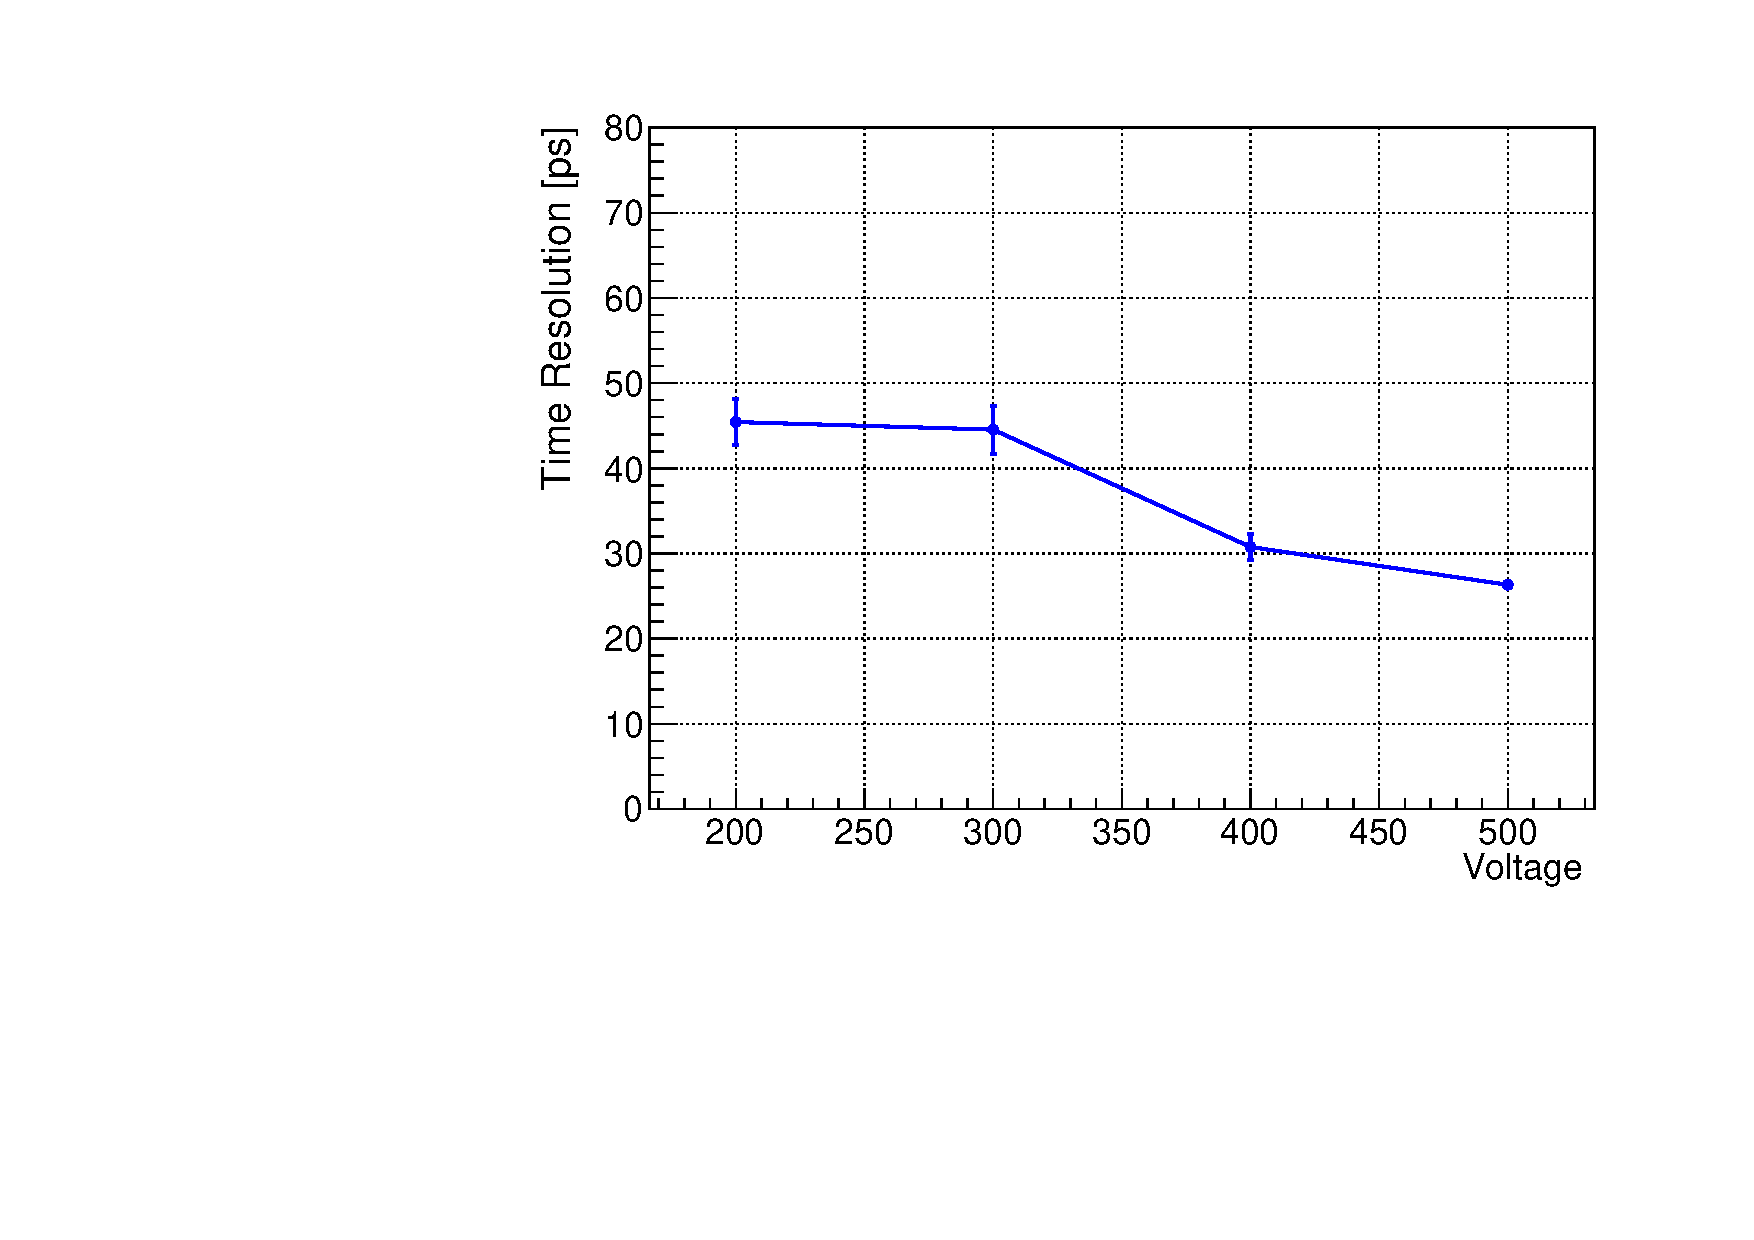
\includegraphics[width=0.8\textwidth]{plots/SigmaT_vs_DV_lin30Stamp.pdf} 
\caption{The time resolution between the silicon sensor and the Photek MCP-PMT 
reference is shown as a function of bias voltage applied on the silicon sensor. } 
\label{fig:SigmaT_vs_DV_lin30Stamp} 
\end{figure} 

\section{Discussion} 
\label{sec:discussion} 

From Figures~\ref{fig:noise}~and~\ref{fig:MIP}, we observe that the noise of the
prototype system is sufficiently low to extract signals from MIPs. Comparing
the RMS of the noise distribution with the mean of the MIP signal, we find a
signal-to-noise ratio around $2$ to $2.5$. A rough estimate from 
Figure~\ref{fig:MIP} demonstrates that the efficiency to detect $120$~GeV protons
and $8$~GeV electrons with no absorber present is larger than $80\%$.
Based on the measurements for MIPs, we derive signal distributions for
electromagnetic showers normalized to MIP response, and observe
a relatively linear response to the electron beam energy after 6 radiation lengths 
of tungsten absorber in Figure~\ref{fig:MIPVsEnergy}. We also measure a 
longitudinal shower profile in Figure~\ref{fig:MIPVsAbsorberAt8GeV} 
that is consistent with similar past measurements. Having established 
standard calorimetric properties of the prototype, we proceed to study 
the timing properties. 

We begin with some general considerations of timing in silicon.
An electric field applied to silicon results in a built-in junction voltage
(~0.6V) which is typical of silicon diodes. The high electric field in silicon
leads to total depletion as all free charge carriers are removed. 
When charged particles pass through the totally depleted region in silicon, 
it ionizes atoms and produces electron-hole pairs which serve as charge carriers.
The electrons are collected on positive electrode and the holes are collected
on the negative electrode. The time and jitter associated with relativistic particles 
traversing through the silicon material can be neglected as it takes 
less than $1$~ps for relativistic particles to pass through the full $300$~$\mu$m
of silicon material. At high electric field (more than $105$~V/cm), the mobility 
of carriers attain a constant drift velocity of $108$~mm/s 
(or about $1\mu$m$/10$~ps) in the silicon material~\cite{Ronzhin2015}. 
The amount of electrons produced in the 100 um is ~10000. The
time needed to collect all electrons in the 100 um is ~1ns. The electrons produced closer to 
the positive electrode collected first. The time needed to pass 1~$\mu$m by electron 
is $\sim$10~ps. The average time between the
electrons is $\sim$1~ps. If electronic can detect 100 electrons its arrival time
could be inside of the 10~ps. The time jitter could be estimated as 3~ps for
Poisson timing distribution. For example, if electronics can detects $\sim$100
electrons (with additional amplification) produced in silicon they collected
from the thickness of $\sim$10~$\mu$m. We can say that the ``rest of the silicon
thickness'' does not participate in the silicon time jitter, because these
electrons are coming ``too late''. This simple model can explain in general
obtained test beam results. 

Our results show that the time stamp associated with electromagnetic 
showers induced by electrons with energy between $20$~GeV and $30$~GeV 
can be measured with a precision better than $25$~ps. Subtracting for the resolution
of the reference Photek MCP-PMT detector yields a precision better than $20$~ps. 
Moreover, we observe an improvement of the time resolution with the energy of 
the electron, and more generally with an increase in the signal amplitude. 
These measurements demonstrate that a calorimeter based on silicon sensors as
the active medium can achieve intrinsic time resolution at the $20$~ps level, as long
as noise is kept under control. Time jitter arising from intrinsic properties of the
silicon sensor is demonstrated to be well below the $20$~ps level.

\section{Conclusion}
\label{sec:conclusion} 

We obtained a best time resolution measurement for silicon sensors of $23$~ps,
using a beam of $32$~GeV electrons and with the silicon sensor placed after 6 radiation
lengths of tungsten absorber. Based on our calibration data for the response of the
silicon sensor to MIPs, this measurement corresponds roughly to 
$54$ secondary particles registered from the electromagnetic shower. 
We observe a roughly linearly increasing response as the energy of the electron beam
is increased, and we observe a longitudinal shower profile consistent with similar 
past measurements. This result yields further encouragement to use silicon as
active layer in calorimeters, as is planned for example for the CMS Phase 2 
upgrade~\cite{Butler:2020886}, and explicitly demonstrates the opportunity 
to use silicon for timing measurements in future calorimeters. In the future, we plan to 
extend our studies to more realistic prototypes covering larger transverse and longitudinal 
regions of the electromagnetic shower and using multiple channels. 


\section{Acknowledgements} We thank the FTBF personnel for very good beam condition during our test beam run. We also appreciate the technical support of the Fermilab SiDet department for the production of high quality silicon samples. We appreciate Helmuth Spieler monography as a good source of silicon information~\cite{spieler2005semiconductor}.

\bibliography{SiliconCalorimeter}{}
\bibliographystyle{ieeetr} 

\end{document}





















